\section{Dark Matter WIMPs}\label{sec:wimps}

% motivating wimps, given the 'wimps are dead' feeling these days
A well-motivated model for particle dark matter is the Weakly Interacting Massive Particle (WIMP)~\cite{Jungman:1995df,Gelmini:2010zh}. While the list of possible dark matter models is now quite long, the WIMP model remains a singularly well-motivated hypothesis, and there are still large regions of well-motivated yet unprobed parameter space~\cite{Arcadi:2017kky}. The hierarchy problem~\cite{Witten:1981nf}, specifically the surprisingly and unnaturally low mass of the Higgs particle, continues to strongly motivate searches for new physics and new particles at the $\sim$100\,GeV scale of the electroweak force~\cite{Tanabashi:2018oca}. This alone would motivate the WIMP hypothesis and WIMP-focused searches, but there is also an additional motivation from what has been termed the `WIMP miracle': if a new stable particle existed in this mass range, and if it interacted with Standard Model particles via some force also at the electroweak scale, then a very simple thermal freeze-out process in the early universe would result in the dark matter density we see in the universe today~\cite{Bertone:2010zza,Steigman:2012nb}. It is this surprising connection of particle physics at the Weak scale and the evolution of the macroscopic density in early cosmology that continues to motivate searches for WIMP dark matter. Few other models can point to as clear a convergence.

% mention of the lee-weinberg limit (by way of later motivating xenon over argon)
The assumption of a massive (electroweak scale) mediator implies a lower bound on the WIMP mass, the so-called Lee-Weinberg limit~\cite{Kolb:1985nn}. A heavy mediator will suppress the dark matter annihilation cross section. Thus, for dark matter with a mass of less than $\sim2$\,GeV$/c^2$, the thermal freeze-out process of the early universe ends too early and results in a dark matter density that is too high and inconsistent with observation.

% mention of complementarity between colliders/indirect/direct
Because WIMPs are so well-motivated, searches for particles satisfying these criteria are underway in parallel following three general and complementary strategies~\cite{Roszkowski:2017nbc} (see also \autoref{sec:complementarity}): 1) production at high energy colliders such as the Large Hadron Collider (LHC)~\cite{Kahlhoefer:2017dnp}; 2) indirectly via annihilation in dense astrophysical environments that produce astrophysical signals in various Standard Model particle channels~\cite{Gaskins:2016cha}; and 3) directly via observation of nuclear recoils produced by dark matter scattering as proposed here~\cite{Undagoitia:2015gya}. The next-generation experiment discussed here is complementary to the next generation of astrophysical searches~\cite{Ong:2017ihp} and the high-luminosity LHC~\cite{Arduini:2016xsb} and at a similar time scale.

% direct detection benefits from being generic and general
Direct detection experiments are particularly interesting for a variety of reasons. As scattering interactions happen at energies far below the electroweak scale itself, the interaction mechanism is simplified and can be described as a contact interaction. A diverse set of high-energy models will therefore appear nearly identical at these low energies with only one characteristic: the scattering cross section. This generality of direct detection via low-energy scattering is a significant advantage to this detection approach. Also, direct dark matter experiments depend only linearly on the local dark matter density, which makes results robust against astrophysical uncertainties. Further, for thermal relics such as WIMPs, the relic density is inversely related to the thermal annihilation cross section, such that a dimensional argument can be made that the expected scattering rate in a detector (which goes like density times cross section) should be roughly independent of details of the theory. 
Another expression of the generality of the direct detection approach is its large mass range of sensitivity~\cite{Smith:1986ms}, almost extending up to the Planck mass (\autoref{sec:planck}). The kinematics for non-relativistic scattering remain unchanged once the WIMP mass is much larger than the target mass, rendering these experiments sensitive to dark matter masses well beyond 100~TeV and even up to the Planck mass~\cite{Bramante:2018qbc} (\autoref{sec:planck}). Thus, a single experiment can probe many orders of magnitude of the allowed dark matter mass parameter space.

% the xenon nucleus is a generally useful one
Xenon in particular is expected to couple well to WIMP dark matter for several reasons. First, in the low momentum-transfer regime of direct detection, a generic spin-independent scattering (\autoref{sec:si}) will interact with the nucleus as a whole as a many-nucleon object, and this coherence provides a significant boost to the corresponding scattering cross section~\cite{Smith:1983jj,Goodman:1984dc}, scaling roughly as the square of the number of nucleons. Therefore, a heavy nucleus like xenon is significantly favored over lighter options. A second advantage is the large number of common natural xenon isotopes, resulting in a diversity of nuclear properties. This variety of isotopes gives xenon significant sensitivity to other interaction models as well, such as spin-dependent (\autoref{sec:sd}) or various effective couplings (\autoref{sec:eft}).

% sensitivity projection method
\autoref{fig:si_sensitivity} on page~\pageref{fig:si_sensitivity} and \autoref{fig:SD_sensitivity} on page~\pageref{fig:SD_sensitivity} show sensitivity estimates for a liquid xenon TPC with only neutrino-induced backgrounds and the double beta decay of ${}^{136}$Xe considered. We use a binned likelihood in position-corrected $cS1$ and $cS2$ (see e.g.~\cite{Akerib:2017vbi,Aprile:2019bbb}), and assume the log-likelihood ratio test statistic is asymptotically distributed~\cite{Wilks:1938dza}. The detector response to electronic and nuclear recoils is simulated using the NEST package~\cite{Szydagis:2021hfh} with the \texttt{LUXrun03} detector model~\cite{szydagis_m_2018_1314669}. The background expectation value is dominated by electronic recoils from naturally occurring $^{136}$Xe and solar (mostly $pp$) neutrinos scattering off electrons. Electronic recoil events can be distinguished from a WIMP signal using the ionization signal. Nuclear recoil events from neutrinos scattering in the detector volume, can be separated to some degree from a WIMP signal based on the recoil energy spectrum and their tendency to scatter multiple times. We include nuclear recoil backgrounds from $^8$B, HEP, diffuse supernovae and atmospheric neutrinos. The recoil spectra, as well as uncertainties on the different components which may significantly affect the sensitivity as neutrinos become the dominant background~\cite{OHare:2020lva}, are taken to be the same as in~\cite{Aprile:2020vtw}, with spectra from~\cite{KotilaIachelloWebSite,Chen:2016eab,Billard:2013qya,Newstead:2020fie}. WIMP recoil spectra are computed using the \texttt{wimprates} package~\cite{wimprates}, with spin-dependent computations from~\cite{Klos:2013rwa}, and WIMP-pion recoil spectra from~\cite{Aprile:2018cxk}. We use the background and signal distributions to construct signal regions for each WIMP interaction and mass. We estimate the region at which neutrinos become an appreciable background as the cross section where the WIMP and neutrino expectation in the signal region are equal. This level is labeled the ``neutrino fog'' in Figures~\ref{fig:si_sensitivity} and~\ref{fig:SD_sensitivity}. 

\subsection{Spin-Independent WIMPs}\label{sec:si}

\begin{figure}[!htbp] 
	\centering
    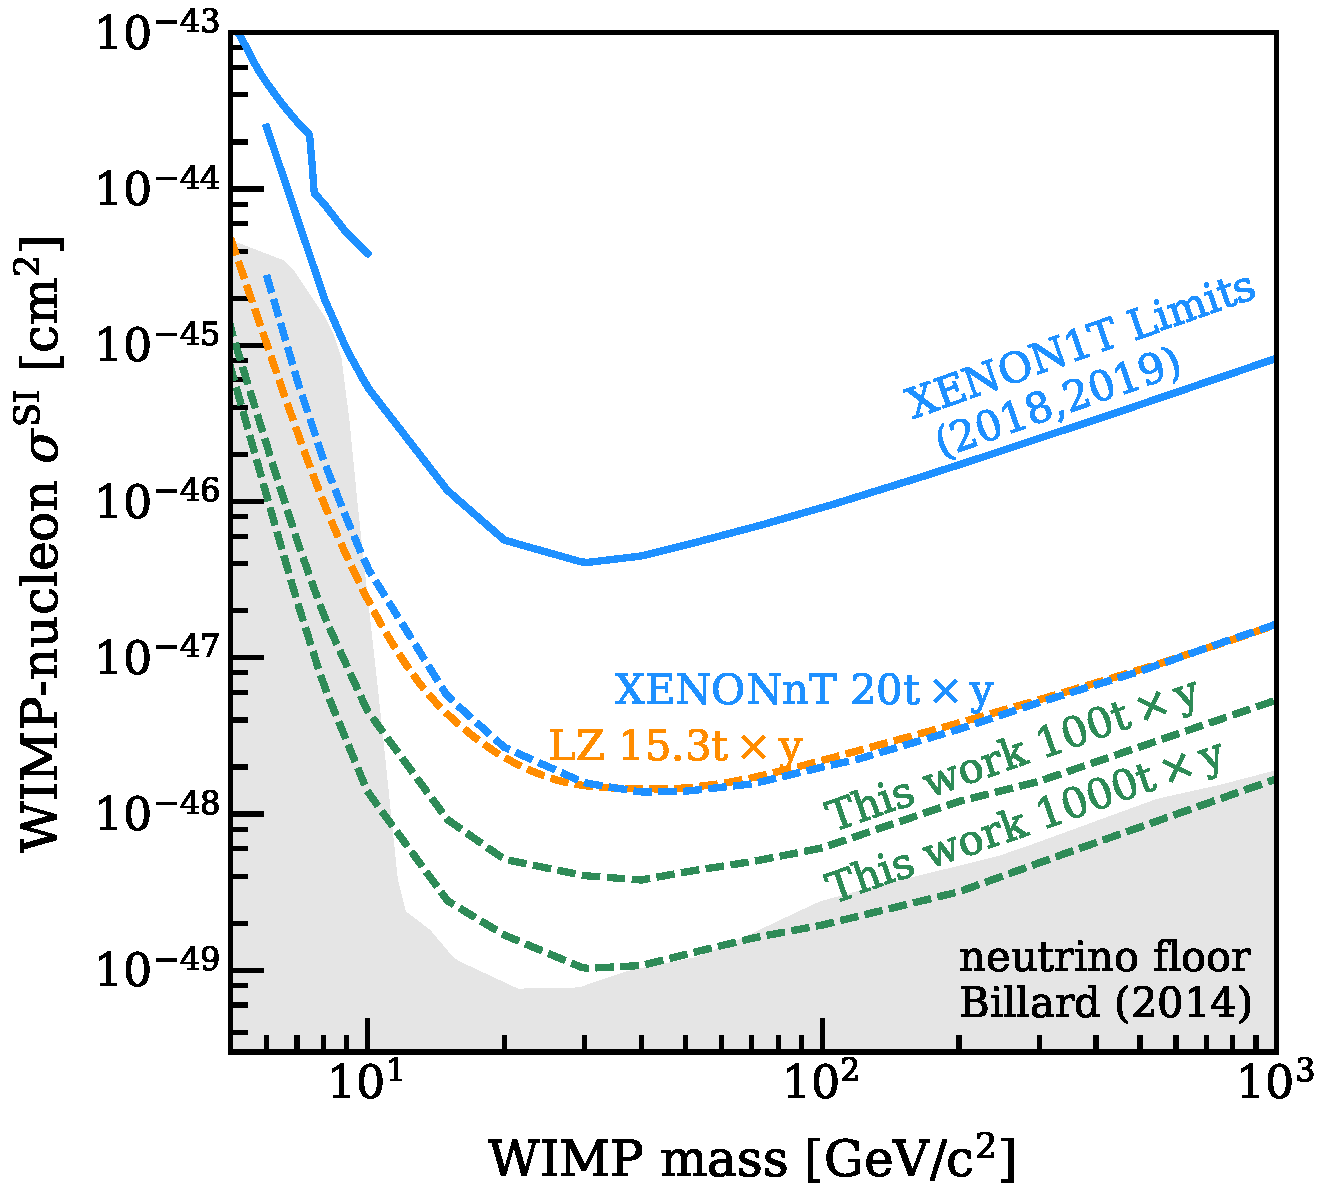
\includegraphics[width=\columnwidth,clip]{fig_simplified_projection_si.pdf}
    \caption{Projections for the next-generation experiment discussed here, together with projected and current leading $90\%$ upper limits, on the spin-independent WIMP-nucleon cross section. Blue solid lines show the current leading limits from XENON1T~\cite{Aprile:2018dbl,Aprile:2019xxb}. Dashed blue and orange lines indicate sensitivity projections from LZ~\cite{Akerib:2018lyp} ($15.3\tonneyear$, one-sided) and XENONnT~\cite{Aprile:2020vtw} ($20\tonneyear$). Projected median upper limits for exposures of $100\tonneyear$ and $1000\tonneyear$ are plotted in dashed green. The shaded gray area indicates where the ``neutrino fog''~\cite{Billard:2014yka} becomes relevant, specifically where more than one neutrino event is expected in the $50\%$ most signal-like S1/S2 region.}
\label{fig:si_sensitivity}
\end{figure}

% why this detector would be 'ultimate' as far as WIMPs are concerned, in both threshold and exposure
The next-generation detector proposed here can be thought of as the `ultimate' WIMP dark matter detector in two senses: exposure and energy threshold. Traditionally, WIMP detection has been limited primarily by the experiment's exposure (expressed in mass $\times$ time), and sensitivity has progressed proportionally to that exposure. This linear scaling will hold as long as contamination by any non-WIMP recoils remains small. This next-generation WIMP detector will be the last to benefit from this proportional scaling over much of its operating time. Any larger experiment would face a rate of coherent elastic neutrino-nucleus scattering from astrophysical sources~\cite{Monroe:2007xp,Billard:2013qya}. While that is an interesting signal in its own right (\autoref{sec:neutrinos}), neutrinos present an unavoidable background to WIMP sensitivity. 

The energy threshold of this search is also important. A recoil threshold of $\sim$keV is required in order to efficiently test WIMP hypotheses of few GeV mass down to the Lee-Weinberg limit. The goal for an ultimate WIMP dark matter detector, then, can be described as testing the entire WIMP mass range ($\sim$2~GeV$/c^2$ -- $\sim$100~TeV$/c^2$) down to cross sections limited by neutrino scattering. Such a detector also has sensitivity to many theoretically interesting and yet unexplored dark matter candidates (\autoref{sec:broaderdarkmatter}) and probes the coupling of dark matter to the Higgs boson~\cite{Feng:2014vea}.

\begin{figure}[!htbp] 
	\centering
    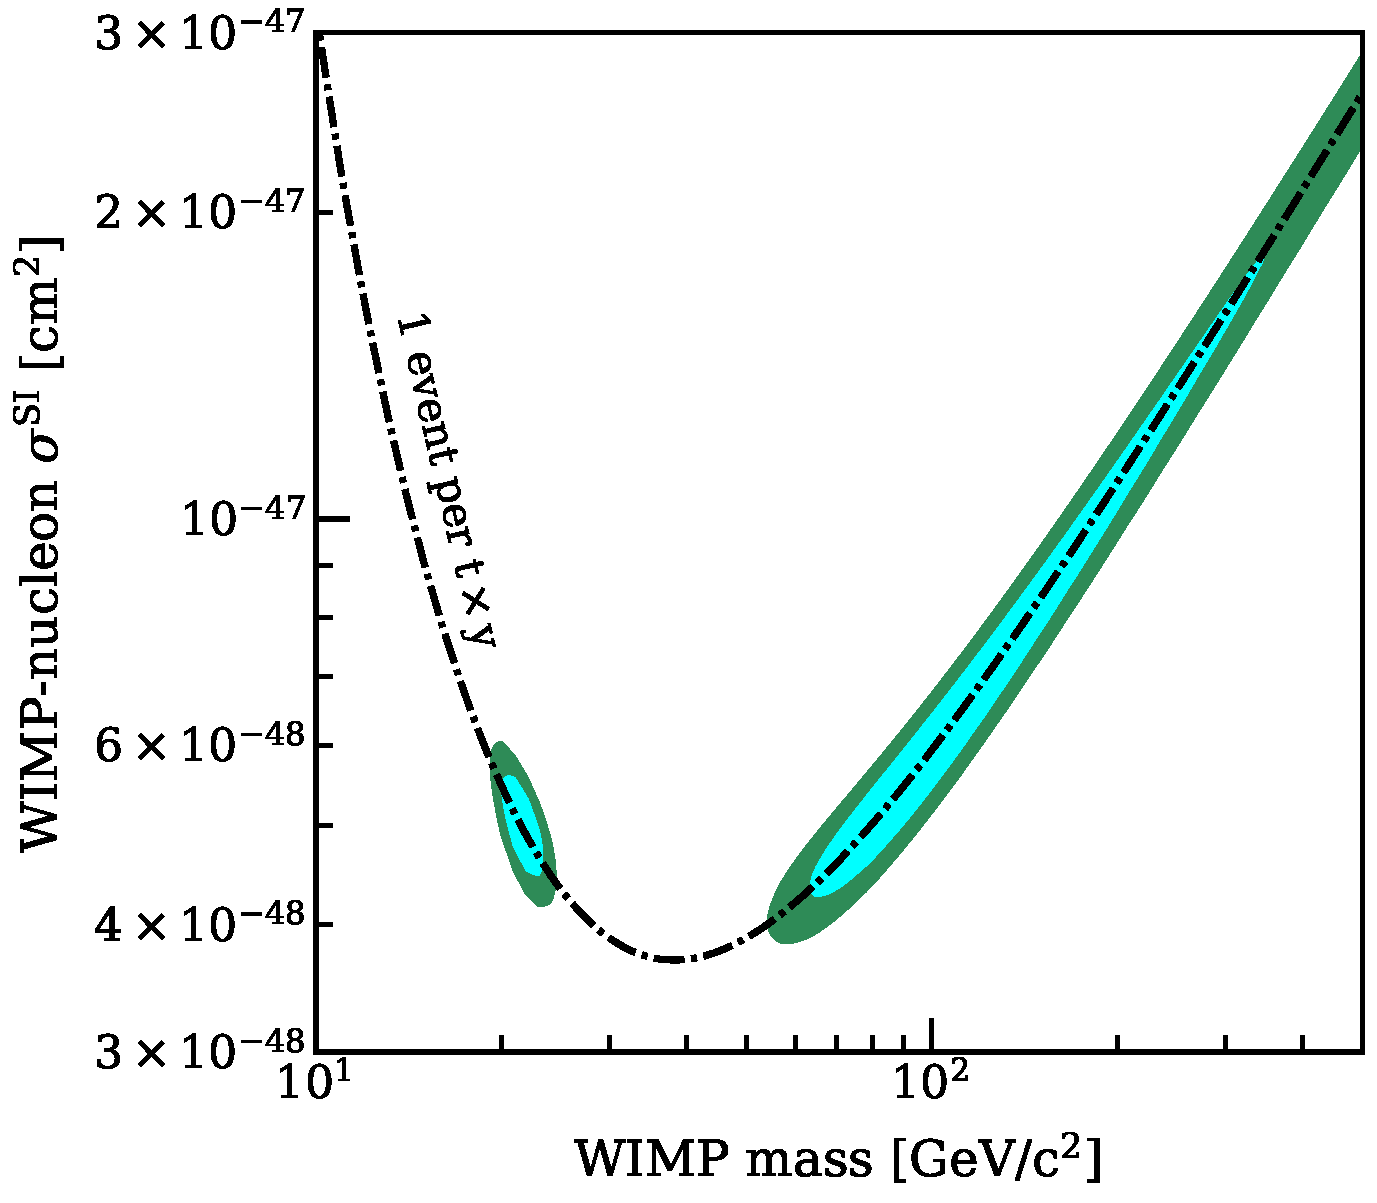
\includegraphics[width=\columnwidth]{fig_simplified_contour_si.pdf}
    \caption{Illustration of 1-~and 2-sigma (cyan and green) confidence intervals on spin-independent WIMP signals with a $1000~\tonneyear$ exposure and WIMP masses of either 20 or $100\1{GeV/c^2}$. The signal expectation for the excesses is $1/\tonneyear$, indicated by the black dash-dotted line}
\label{fig:excess_contour}
\end{figure}

To indicate the WIMP mass and cross section resolution expected for a signal from WIMPs roughly one order of magnitude below current constraints (one event per tonne-year), \autoref{fig:excess_contour} shows confidence intervals for spin-independent WIMP signals at 20 and $100\1{GeV/c^2}$. At high masses, spin-independent WIMP spectra are degenerate in WIMP mass (as the kinematics only depend on the reduced mass). This leads to poor mass resolution, which can be significantly improved using additional, different target materials~\cite{Pato:2010zk}. An excess for intermediate and low masses will be well-constrained both in mass and cross section using a xenon target alone.

\subsection{Spin-Dependent Scattering}\label{sec:sd}

\begin{figure}[!htbp] 
	\centering
    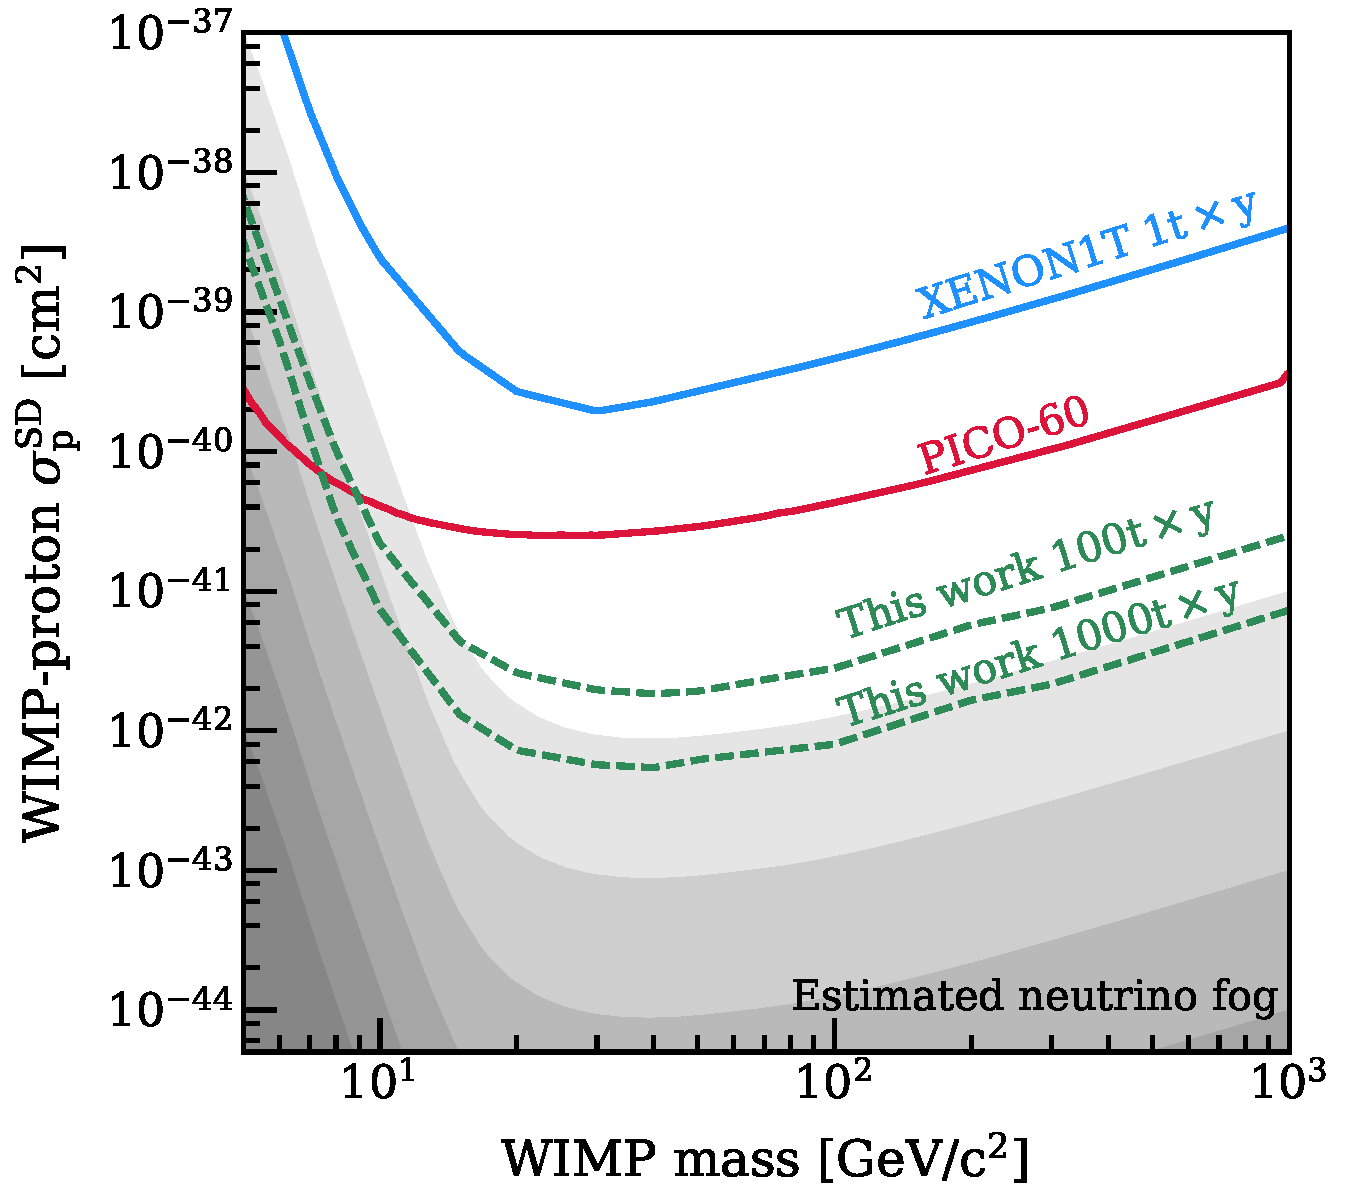
\includegraphics[width=\columnwidth,clip]{fig_simplified_projection_sdp.pdf}
    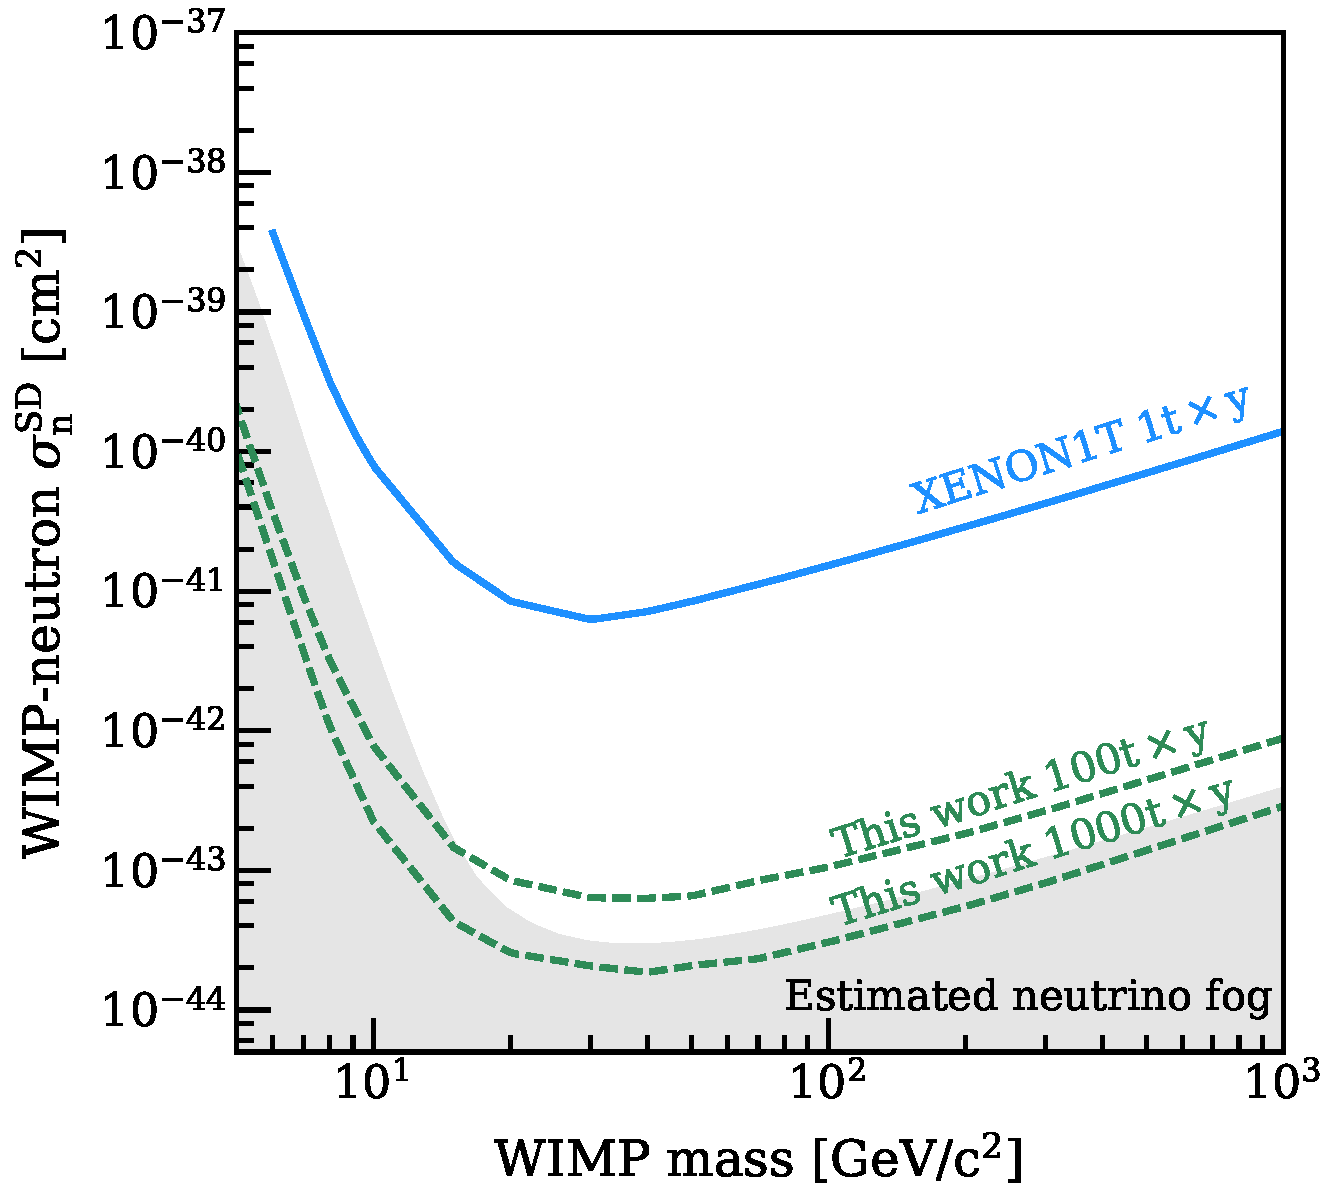
\includegraphics[width=\columnwidth,clip]{fig_simplified_projection_sdn.pdf}
    \caption{Projections and current leading $90\%$ upper limits on the spin-dependent WIMP-nucleon cross section. Blue and red solid lines show the current leading limits by PICO-60~\cite{Amole:2017dex} and XENON1T~\cite{Aprile:2018dbl,Aprile:2019xxb}. Projected median upper limits for exposures of $100\tonneyear$ and $1000\tonneyear$ are plotted in green. The shaded gray areas indicate the ``neutrino fog'' with the lightest area showing the WIMP cross section where more than one one neutrino event is expected in the $50\%$ most signal-like $S1,S2$ region. Subsequent shaded areas indicate tenfold increases of the neutrino expectation.}
\label{fig:SD_sensitivity}
\end{figure}

% spin-dependency, proton/neutron only
The simplest deviation from the spin-independent scattering to a more complicated coupling can be modeled by allowing the WIMP coupling to protons and neutrons to be different while interacting solely with the nuclear spin. This scenario is typically referred to as spin-dependent scattering~\cite{Engel:1992bf,Tovey:2000mm}. The interaction strength can then depend on the nucleon type, i.e.~proton or neutron, and the coupling strengths $f_p, f_n$ can be non-trivial. If one simplifies this picture by assuming that one coupling vanishes, then the derivation of a differential rate of scattering events by WIMPs depends on the spins and nuclear structure (mostly of the unpaired nucleon) of the nuclei in the target. 

% xenon rocks; sensitivity projection
For xenon detectors, the two naturally occurring isotopes $^{129}$Xe (spin-1/2) and $^{131}$Xe (spin-3/2), with natural abundances of 26.4\% and 21.2\%, respectively, are most relevant for this spin-dependent coupling. Both have an unpaired neutron, making xenon also an ideal target for detecting the spin-dependent WIMP-neutron cross section. The projected sensitivity for a next-generation liquid xenon TPC is shown in \autoref{fig:SD_sensitivity}, calculated using the same assumptions and method as in \autoref{fig:si_sensitivity}.

\subsection{Effective Field Theory}\label{sec:eft}

The spin-independent and spin-dependent scattering discussed in the previous sections~\ref{sec:si} and~\ref{sec:sd} are the more frequently studied interactions of the WIMP with Standard Model fields. Their motivation dates back to dark matter candidates in supersymmetric theories~\cite{Engel:1992bf} defining the leading responses related to the nuclear density (therefore scaling coherently with the number of nucleons $A$, spin-independent interactions) or to the nuclear spin (spin-dependent interactions). A more systematic picture covering more general WIMP-nucleus interactions beyond standard spin-independent and spin-dependent scattering has been worked out recently using effective field theories (EFTs). This includes both a nonrelativistic framework, see \autoref{sec:nreft}, as well as chiral effective field theory, see \autoref{sec:cheft}, which incorporates the constraints from QCD at low energies.

\subsubsection{Nonrelativistic Effective Field Theory}\label{sec:nreft}

The nonrelativistic EFT (NREFT)~\cite{Fan:2010gt,Fitzpatrick:2012ix,Anand:2013yka} integrates out all degrees of freedom except for nucleons and the WIMP. The effective operators that describe the coupling of the WIMP to nucleons are constructed imposing Galilean invariance in terms of the momentum transfer $q$, the WIMP transverse relative velocity $v^\perp$, and the spins of the nucleon and the WIMP~\cite{Fitzpatrick:2012ix,Anand:2013yka}. At lowest order in $q$ and $v^\perp$, the only contributions correspond to the leading operators considered for spin-independent and spin-dependent scattering. Up to second order in $q$ and first order in $v^\perp$, 14~operators appear at the single-nucleon level for spin-1/2 dark matter, each with different isoscalar and isovector (or, equivalently, proton and neutron) couplings~\cite{Anand:2013yka}. The corresponding coefficients, usually considered to be independent, have been constrained from several experiments~\cite{Schneck:2015eqa,Aprile:2017aas,Xia:2018qgs,Angloher:2018fcs}. With few exceptions, the best constraints are given by experiments using a xenon target. For an extension of NREFT to dark matter of spin 1 or higher, see~\cite{Dent:2015zpa,Catena:2019hzw,Gondolo:2020wge}.

Since the NREFT is limited to nucleons as degrees of freedom, additional matching steps are required to constrain particular WIMP models from experimental limits. This is because the NREFT coefficients contain information on the underlying WIMP-quark or WIMP-gluon operators, but also on hadronic matrix elements (\autoref{sec:structure}). In addition, there is a~priori no hierarchy among the various NREFT operators apart from their scaling in $q$ and $v^\perp$. In that sense, the NREFT can be considered minimal, as even constraints from QCD are not imposed. In addition, the NREFT formalism has also been used to represent contributions beyond the applicability of the strict EFT. For example, long-range effects due to pion exchange (as occurs in chiral EFT) or electromagnetic interactions (such as dipole operators) can be expressed in terms of $q$-dependent NREFT Wilson coefficients. For a complete description, however, the corresponding degrees of freedom need to be included in the EFT.  

\subsubsection{Chiral Effective Field Theory}\label{sec:cheft}

Chiral EFT~\cite{Epelbaum:2008ga,Machleidt:2011zz,Hammer:2012id} classifies the possible interactions of the WIMP with nucleons according to their chiral scaling, i.e., the scaling with momenta and quark masses, with nucleons and WIMPs but also pions (and, in SU(3), kaons and $\eta$-mesons) as active degrees of freedom. In this way, the constraints from the chiral symmetry of QCD are automatically included. The chiral regime is appropriate to study WIMP-nucleus scattering because the typical momentum transfer $q$ is of the order of the mass of the pion, the pseudo-Nambu-Goldstone boson resulting from the spontaneous breakdown of chiral symmetry. This is also the relevant scale for the heavier nuclei, such as xenon, used for direct detection experiments.

At the single-nucleon level, the chiral analysis can be mapped onto the NREFT operator basis~\cite{Hoferichter:2015ipa,Bishara:2016hek,Bishara:2017pfq}. This provides a prediction for an additional hierarchy of the NREFT operators based on their chiral scaling, which significantly simplifies the number of one-body operators relevant for WIMP-nucleus scattering. A second important advantage of the chiral EFT framework is that it predicts subleading multi-nucleon effects. For example, contributions in which the WIMP couples to a virtual pion exchanged between the nucleons inside the nucleus (\autoref{sec:wimp_pion}) appear at subleading order in the chiral expansion. Such meson-exchange currents (or two-body currents) provide subleading contributions to generalized spin-independent and spin-dependent scattering and have been studied in a number of papers~\cite{Prezeau:2003sv,Cirigliano:2012pq,Menendez:2012tm,Klos:2013rwa,Cirigliano:2013zta,Hoferichter:2015ipa,Hoferichter:2016nvd,Korber:2017ery,Hoferichter:2017olk,Andreoli:2018etf,Hoferichter:2018acd}. For a xenon target, two-nucleon currents improve the sensitivity to spin-dependent WIMP-proton scattering by more than an order of magnitude.

\subsubsection{WIMP-Pion Coupling}\label{sec:wimp_pion}

A novel contribution to WIMP-nucleus scattering that emerged from the chiral EFT analysis (\autoref{sec:cheft}) concerns meson-exchange currents. In the simplest case, the WIMP couples to a virtual pion exchanged between two nucleons within the nucleus. Interestingly, meson-exchange contributions, which enter at subleading order in chiral EFT, can scale coherently with the number~$A$ of nucleons. The combination of the nuclear and chiral hierarchies defines a scaling that lies between the spin-independent and spin-dependent responses, coherent but suppressed in the chiral counting. Chiral EFT also predicts the leading meson-exchange currents to dominate over all other NREFT operators except the standard spin-independent one.

As observed in~\cite{Aprile:2018cxk}, once an underlying quark-level operator is specified, the resulting limits can be expressed in terms of a WIMP-pion cross section, in close analogy to the spin-independent and spin-dependent WIMP-nucleon cross sections. The proposed next-generation liquid xenon experiment will improve this result by a similar factor as the standard spin-independent limit, shown in \autoref{fig:wimppion_sensitivity}.

\begin{figure}[!htbp] 
	\centering
    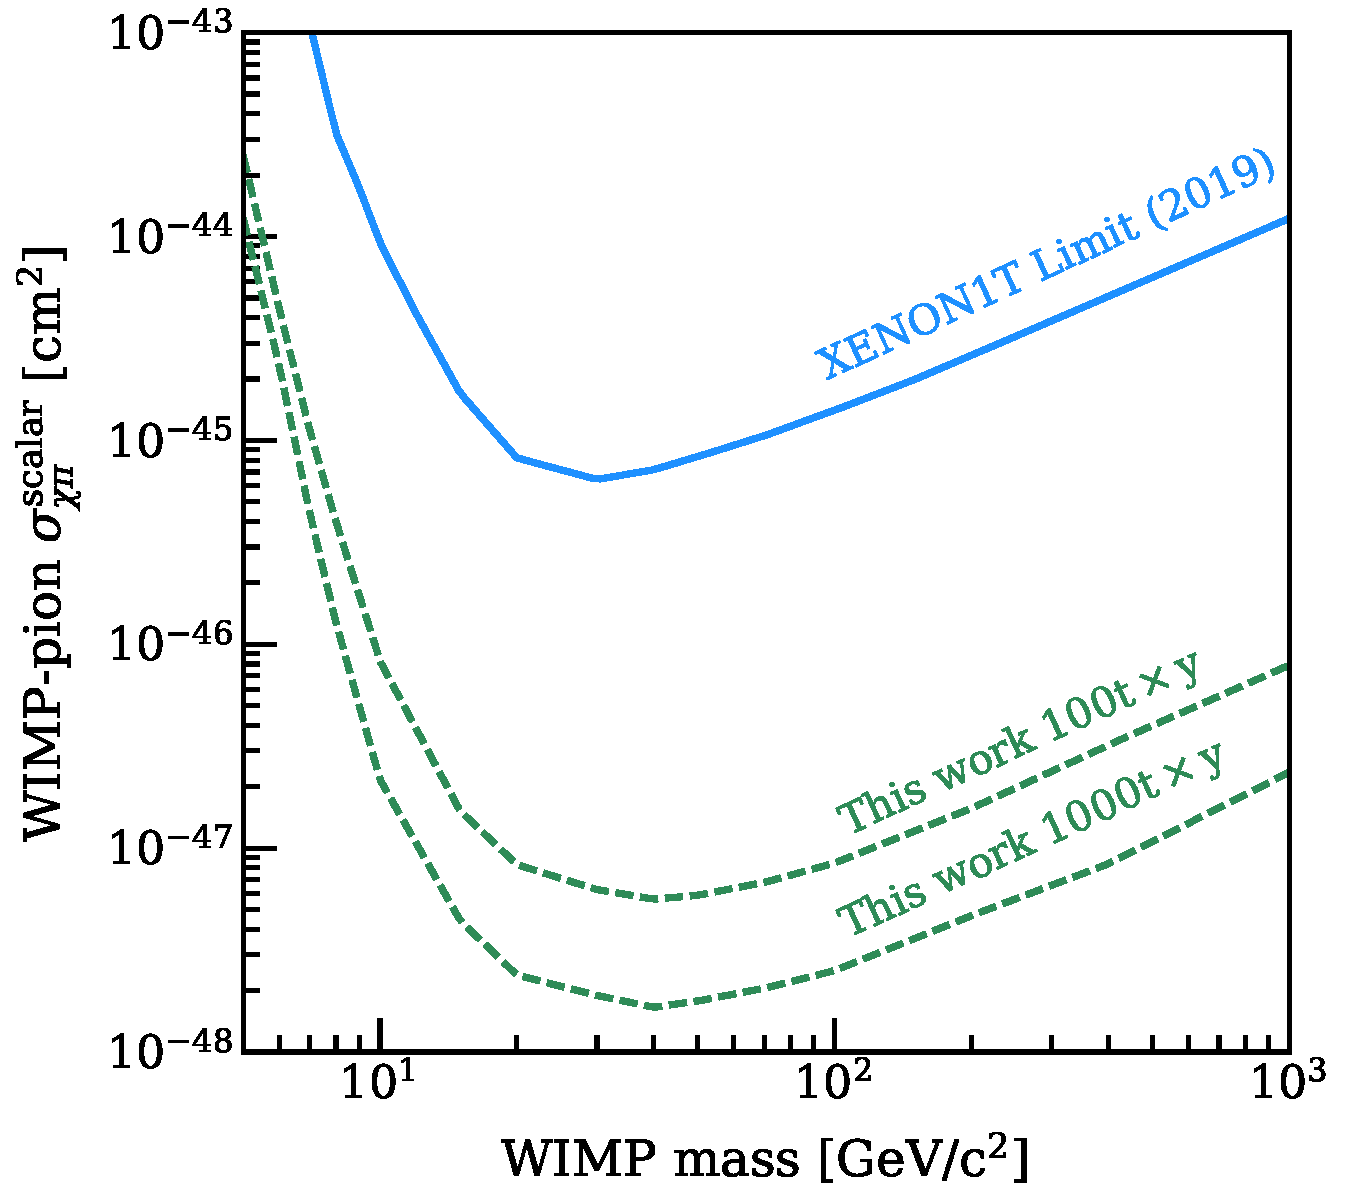
\includegraphics[width=\columnwidth,clip]{fig_simplified_projection_pion.pdf}
    \caption{Projections and current leading $90\%$ upper limits on the scalar WIMP-pion interaction cross section. Blue solid lines show the current leading limits by XENON1T~\cite{Aprile:2018cxk}. Projected median upper limits for exposures of $100\tonneyear$ and $1000\tonneyear$ are plotted in green.}
\label{fig:wimppion_sensitivity}
\end{figure}

\subsubsection{Three-Flavor EFT and the UV}\label{sec:quark-level}

From a particle physics point of view, the most immediate parameterization of dark matter interactions at low energies, $\mu\simeq 2$ GeV, is in terms of three-flavor dark matter EFT that has been studied extensively~\cite{Goodman:2010yf,Goodman:2010ku,Fox:2011pm,Crivellin:2014qxa,DEramo:2014nmf,Hill:2014yxa,Hill:2014yka,Bishara:2016hek,Bishara:2017pfq,Bishara:2017nnn,Brod:2017bsw,Hoferichter:2015ipa,Hoferichter:2016nvd,Hoferichter:2018acd}. This model has as degrees of freedom the dark matter particle, the lightest three flavors of quarks ($u,d,s$), the gluon, and the photon. Dark matter interactions are organized in terms of dimensions of the operators, so that the effective Lagrangian takes the form ${\cal L}_{\rm DM~EFT}= \sum_{d,a} {\cal C}_a^{(d)} {\mathcal Q}_a^{(d)} / \Lambda^{d-4} $, where ${\cal C}_a^{(d)}$ are dimensionless Wilson coefficients and $\Lambda$ the typical scale of the UV theory for dark matter. The sum is over different types, $a$, and dimensions, $d$, of the operators ${\mathcal Q}_a^{(d)}$. An example of a dimension-6 operator for fermionic dark matter is $(\bar \chi \gamma^\mu \chi)(\bar q\gamma_\mu q)$ for dark matter-quark vector interactions, or a dimension-7 operator $m_q(\bar \chi \chi)(\bar q q)$ for scalar interactions, both of which lead to spin-independent scattering. The full basis of up to and including dimension-7 operators in the limit $\Lambda \gg m_\chi \sim m_W$ can be found in~\cite{Brod:2017bsw}. The case of the heavy dark matter limit is discussed in~\cite{Hill:2011be,Hill:2014yka,Hill:2014yxa,Chen:2019gtm}). The chiral EFT of \autoref{sec:cheft} then gives the hadronization of the three-flavor dark matter EFT and the nuclear response.

The three-flavor dark matter EFT is a valid description for dark sector mediators that are heavier than a few hundred MeV. In this case, the mediators are heavier than the typical momenta exchanged in the dark matter scattering on nuclei and can be integrated out. The Wilson coefficients, ${\cal C}_a^{(d)}$, are constants that contain all the UV dark matter physics. In the absence of a complete UV theory of dark matter they can be freely varied when comparing the results of dark matter direct detection experiments. For $\Lambda$ well above the nuclear scale, the higher dimension operators are suppressed, making the framework predictive. For instance, for $\Lambda \gg m_\chi$,  a truncation at dimension~7 is expected to capture most new physics models.

The connection between the three-flavor dark matter EFT at $\mu =2\1{GeV}$ and the UV theory at $\mu \simeq \Lambda$ is achieved by going through a series of appropriate EFTs and performing the matchings at each threshold~\cite{Crivellin:2014qxa,Brod:2018ust,Bishara:2018vix,DEramo:2014nmf,Crivellin:2014gpa}. In this way the results of indirect dark matter searches and the dark matter searches at the LHC can be reliably compared with the direct detection results. From the perspective of direct detection experiments, the UV physics is encoded in the values of Wilson coefficients ${\cal C}_a^{(d)}$. One can then compare the constraints on ${\cal C}_a^{(d)}$ obtained from direct detection experiments with the constraints imposed by the LHC and indirect dark matter searches on either complete dark matter models or on simplified models by going through the above series of matchings and renormalization group evolutions. 

\subsection{Nuclear Structure Factors}\label{sec:structure}

The WIMP-nucleus cross section is proportional to the nuclear structure factors, which encode the relevant information of the structure of the target nuclei. The EFT operators at the WIMP-nucleon level generate, at the nuclear level, six different nuclear one-body responses analogous to semileptonic weak interactions~\cite{Serot:1978vj,Donnelly:1979ezn,Serot:1979yk}. In addition, chiral EFT predicts two-nucleon nuclear responses associated with meson-exchange currents. The corresponding nuclear structure factors are obtained from the one-body nuclear responses $\mathcal{F}^M$, $\mathcal{F}^{\Phi ''}$, $\mathcal{F}^{\Sigma '}$, $\mathcal{F}^{\Sigma ''}$, $\mathcal{F}^{\tilde{\Phi} '}$, and $\mathcal{F}^{\Delta}$~\cite{Engel:1992bf,Anand:2013yka}, and the two-body nuclear responses $\mathcal{F}_{\pi}$, $\mathcal{F}_{\rm b}$~\cite{Hoferichter:2016nvd,Hoferichter:2018acd}. The one-body structure factors decompose into isoscalar and isovector (or, equivalently, proton and neutron) contributions, e.g., $\mathcal{F}^M_\pm$. $\mathcal{F}^M$ and the two-body $\mathcal{F}_{\pi}$, $\mathcal{F}_{\rm b}$ can receive coherent contributions from all $A$ nucleons in the nucleus while about one in five nucleons contributes coherently to $\mathcal{F}^{\Phi ''}$. These responses dominate spin-independent ($\mathcal{F}^M$) and scalar WIMP-pion ($\mathcal{F}_{\pi}$) scattering. $\mathcal{F}^{\Sigma '}$ and $\mathcal{F}^{\Sigma ''}$ are usually rewritten in terms of the more common $S_{00}$, $S_{01}$, $S_{11}$ or $S_p$, $S_n$ in spin-dependent analyses. They are related to the spin distribution in the nucleus and are not coherent because the nuclear pairing interaction couples nucleons in spin-zero pairs.

The nuclear structure factors allow one to factorize the nuclear response from the hadronic matrix elements and the couplings of the WIMP. Schematically, the WIMP-nucleus cross sections decomposes as
\begin{equation}
 \frac{{\rm d}\sigma_{\chi\mathcal{N}}}{{\rm d}q^2}\propto \sum_i \big|c_i \mathcal{F}_i(q^2)\big|^2 + {\rm interference\ terms},
\end{equation}
where the $\mathcal{F}_i(q^2)$ denote the nuclear structure factors and the $c_i$ involve a convolution of hadronic matrix elements and WIMP couplings. In special cases, the WIMP-nucleus cross section can be expressed in terms of single-particle cross sections: (i) if only $c^M_+$ is non-vanishing it can be expressed by the spin-independent isoscalar WIMP-nucleon cross section (\autoref{sec:si}); (ii) if only the coefficients of $S_p$ or $S_n$ are non-vanishing, by the spin-dependent WIMP-proton or WIMP-neutron cross section (\autoref{sec:sd}); and (iii) if only $c_\pi$ is non-vanishing, by the scalar WIMP-pion cross section (\autoref{sec:wimp_pion}).

\begin{figure}[!htbp] 
\centering
	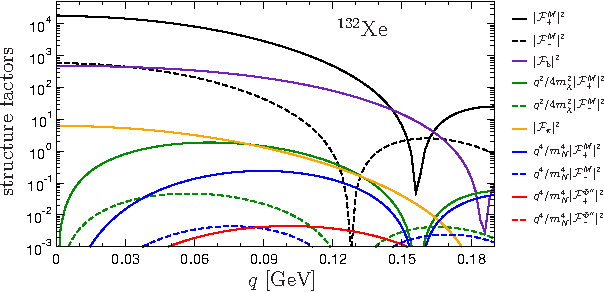
\includegraphics[width=\columnwidth,clip]{fig_structure_factors_xe132.pdf}
	\caption{Structure factors for $^{132}$Xe from one- and two-body contributions (without interference terms). Solid lines show isoscalar and two-body contributions while dashed lines indicate isovector couplings. Figure taken from~\cite{Hoferichter:2018acd}.}
	\label{fig:structure_factors_xe132}
\end{figure}

In general, reliable nuclear structure factors for any nuclear response require a good description of the nuclear target. The only exception is the leading $\mathcal{F}^M_+$ structure factor in spin-independent scattering, for which the purely phenomenological Helm form factor~\cite{Helm:1956zz,Lewin:1995rx} is a common and accurate description~\cite{Vietze:2014vsa}. For heavy targets such as xenon, structure factors need to be calculated from nuclear theory. The nuclear shell model is presently the method of choice with significant progress in recent years. The shell model solves the many-body problem in a relatively small configuration space (one or two harmonic oscillator shells near the Fermi surface) with a phenomenological nuclear interaction adapted to the configuration space~\cite{Caurier:2004gf}. The description of excitation energies, charge radii, and electromagnetic properties of medium- and heavy-mass nuclei, including all stable xenon isotopes, is already very good~\cite{Hoferichter:2018acd,Vietze:2014vsa,Klos:2013rwa}. State-of-the-art nuclear structure factors are easily available in dedicated notebooks documented in~\cite{Hoferichter:2018acd,Anand:2013yka}. \autoref{fig:structure_factors_xe132} shows nuclear structure factors for a general coherent WIMP scattering off $^{132}$Xe (26.9\% natural abundance) with the hierarchy given by chiral EFT.

More advanced nuclear structure {\it ab initio} calculations treat explicitly all nucleons in the nucleus~\cite{Punjabi:2015bba,Navratil:2016ycn}. They can use nuclear interactions based on chiral EFT, thus consistently providing the nuclear states and WIMP-nucleon operators that enter the calculation of the structure factors. This will allow one to estimate theoretical uncertainties. While nuclear structure factors obtained with {\it ab initio} many-body techniques have historically been limited to light nuclei with $A \leq 6$~\cite{Friar:1993kk,Kamada:2001tv,Gazda:2016mrp,Andreoli:2018etf,Korber:2017ery}, recent progress has been significant and made these calculations applicable to nuclei as heavy as nickel~\cite{Hagen:2010zz,Hagen:2012fb,Hergert:2013uja,Hagen:2015yea,Navratil:2016ycn}.

\subsection{Inelastic Scattering}\label{sec:inelastic}

The recoil energy spectrum resulting from spin-dependent interactions is similar to the one expected from spin-independent interactions. Using different target materials with other experiments can help to break that degeneracy, as would be a different mixture of isotopes of xenon in a target. In addition, liquid xenon TPCs can even differentiate between these two interaction channels with one and the same exposure, as WIMPs might alternatively scatter inelastically off nuclei that possess low-lying excited states up to $\sim$100 keV, including $^{129}$Xe and $^{131}$Xe~\cite{Baudis:2013bba,Aprile:2017ngb,Aprile:2020sfu}. This inelastic scattering in the nuclear sector is not to be confused with dark matter models in which the WIMP can be excited, as is discussed in the context of the inelastic Dark Matter (iDM) model in \autoref{sec:inelasticdarkmatter}. 

Inelastic scattering is always non-coherent, because of the different initial and final nuclear states. This would allow one to narrow the nature of the underlying WIMP-nucleon interaction, testing the spin-dependent case upon detection in the simplest scenario. In addition to the nuclear recoil, a prompt electronic recoil is caused by the de-excitation of the up-scattered xenon nucleus. Such interactions thus suffer from the larger background of electronic recoils. However, since they would only be expected for non-coherent spin-dependent interactions, given sufficient statistics, a single xenon detector would be able to extract information about dark matter that is inaccessible to the elastic channel alone. 

Observation of such inelastic scattering would provide a range of further insights to the nature of dark matter: Each unique nuclear excitation is sensitive to a distinct portion of the WIMP halo, so that multiple contributions from the inelastic channel could be combined with that of the elastic channel to constrain the WIMP velocity distribution~\cite{Baudis:2013bba}. In addition, the range of observed recoil energies as well as the energy at which the inelastic channel begins to overtake the elastic one would indicate the mass of the incident WIMP. Finally, in contrast to the elastic channel, the inelastic event rate may be enhanced or suppressed with the enrichment or depletion of $^{129}$Xe and $^{131}$Xe. This flexibility would allow one to optimize data acquisition in a xenon detector. The most stringent limit on inelastic WIMP-nucleon scattering currently comes from the XMASS detector~\cite{Suzuki:2019ine}. Prospects for a future detection of dark matter detection with inelastic xenon transitions are further discussed in~\cite{McCabe:2015eia}.

\subsection{Discriminating Between WIMP-Nucleus Responses}

Given the number of different nuclear responses (\autoref{sec:structure}), a key question is how they could, in the event of a detection, be distinguished in order to extract information on the nature of the WIMP. One possible strategy concerns the study of inelastic scattering into low-lying excited states of the xenon target, discussed in the previous \autoref{sec:inelastic}. The detection of the inelastic channel, in addition to the elastic scattering would primarily point to the non-coherent character of the WIMP-nucleus interaction, suggesting a spin-dependent interaction as the prime choice.

\begin{figure}[!htbp] 
	\centering
	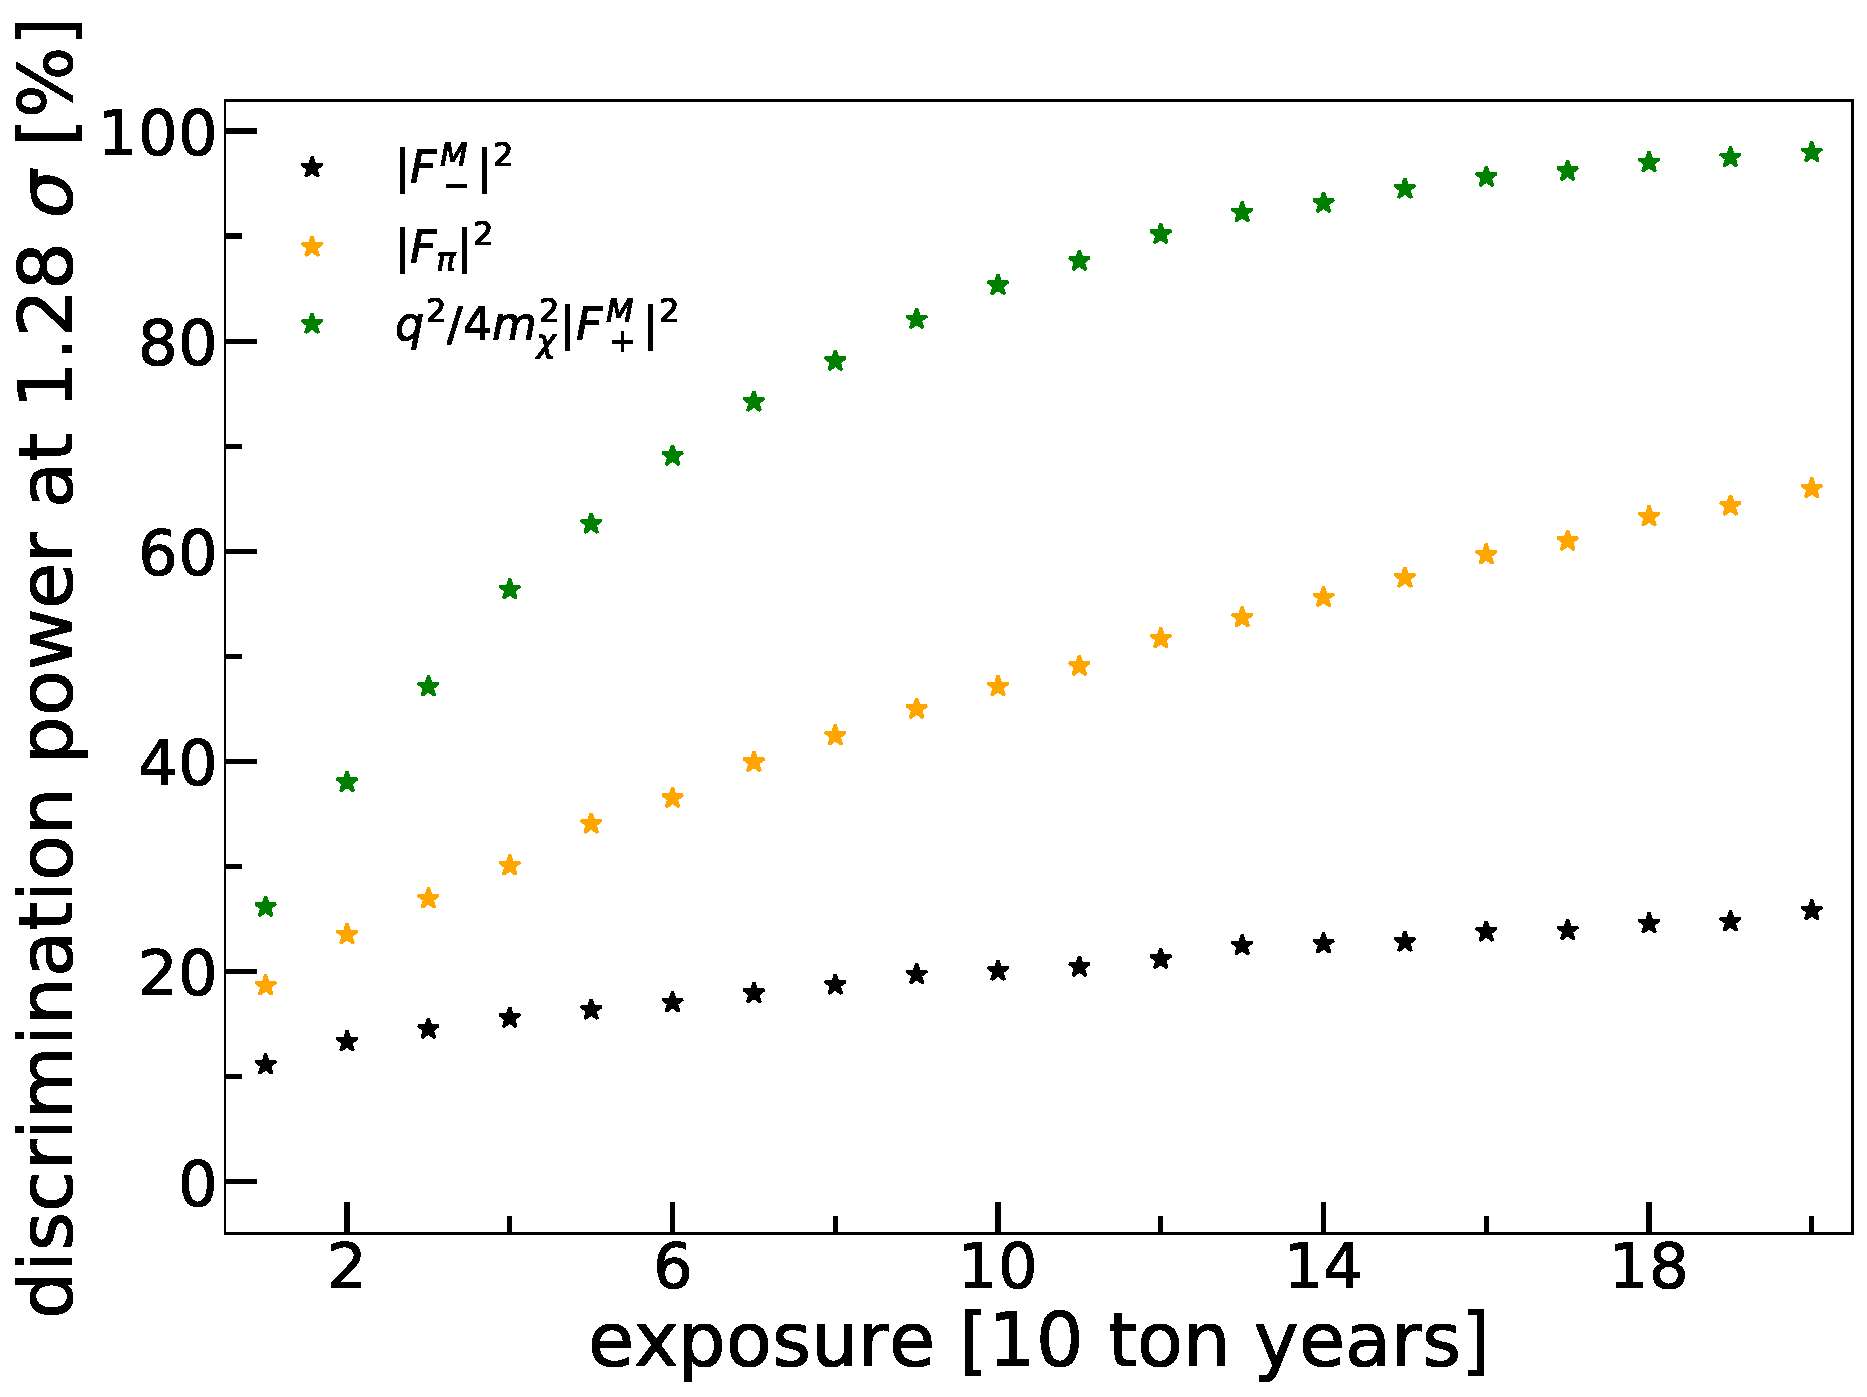
\includegraphics[width=\columnwidth]{fig_results_exp_new_leg.pdf}
	\caption{Discrimination power against $|\mathcal{F}_+^M|^2$ vs.\ exposure for three selected structure factors, $|\mathcal{F}_-^M|^2$ (black), $|\mathcal{F}_\pi|^2$ (orange), and $q^2/4m_\chi^2 |\mathcal{F}_-^M|^2$ (green). 
	The detector setting is like the one discussed here, for a WIMP mass of $m_\chi =100$ GeV$/c^2$ and interaction strength $\sigma_0=10^{-47}\,{\rm cm}^2$. Figure taken from~\cite{Fieguth:2018vob}.} 
	\label{fig:results_example}
\end{figure}

A second handle to discriminate the nuclear responses exploits their different dependence on the momentum transfer, see \autoref{fig:structure_factors_xe132}. The feasibility of this approach has been explored for several WIMP-nucleon interactions~\cite{Fieguth:2018vob,Rogers:2016jrx}. In particular, Ref.~\cite{Fieguth:2018vob} considered realistic detector settings, including projections for a next-generation experiment like the one proposed here, see \autoref{fig:results_example}. As with inelastic scattering, for most responses a discrimination becomes possible with sufficient statistics. However, due to the similarities in the $q$-dependence, a separation of isoscalar and isovector responses will be difficult.

Finally, the nature of the WIMP-nuclear response and in particular its spin-dependent character can be tested by varying the enrichment or depletion on the isotopes with odd $A$ $^{129}$Xe and $^{131}$Xe that is possible with a liquid xenon target. In this case it will be most powerful to combine the results of the proposed experiment with searches using spinless nuclear targets, such as argon, to further test the spin-dependent hypothesis. Likewise, to discriminate between isoscalar and isovector responses the most promising strategy takes advantage of the different proton to neutron ratios in different target nuclei. In this sense, xenon isotopes exhibit the smallest proton to neutron ratios, in contrast to the largest ones which are found e.g.~in fluorine or argon.

\subsection{Scattering at High Momentum Transfer}

Traditional momentum- and velocity-independent dark matter models used to drive experimental developments already starting in the 1990s. Those lead to the well-known low-energy recoil spectra, resembling simple distributions exponentially falling with energy~\cite{Lewin:1995rx}. Consequently, significant experimental effort went into lowering the energy threshold, the calibration for nuclear recoils in this energy regime, and improved understanding of relevant background sources. 

However, many models, such as momentum-dependent effective models or non-trivial mixtures of interactions, result in a more complex nuclear recoil signature with characteristic peaks in the higher nuclear energy regime. This includes many of the models discussed in the following, such as inelastic, exothermic, and magnetic dark matter~\cite{Schneck:2015eqa,TuckerSmith:2001hy, Graham:2010ca, Dienes:2014via, Bramante:2016rdh} but also the well-known EFT operators for elastic scattering~\cite{Gluscevic:2015sqa, Aprile:2017aas,Gelmini:2018ogy}. These effects manifest themselves often outside the traditionally analyzed energy ranges. The fact that most particles in the Standard Model adhere to such more complex interactions provides strong motivation to explore this important higher-energy parameter space. \autoref{fig:high_nr_spectra} show possible recoil spectra for selected interactions, taken from~\cite{Bozorgnia:2018jep}. Further motivation to also probe higher recoil energies stems from the presence of Galactic streams that may result in higher recoil energies than from the customarily assumed isothermal halo~\cite{Freese:2003tt,Helmi:2004id,Vogelsberger:2007ny,Kuhlen:2009vh,Lang:2010cd,Purcell:2012sh,Buckley:2019skk}. 

\begin{figure}[!htbp]
\centering
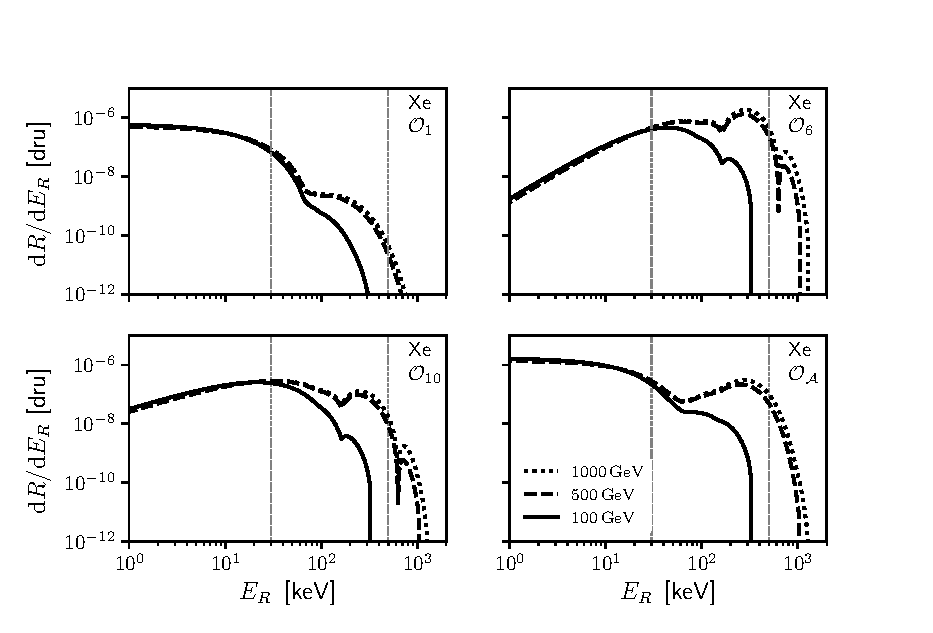
\includegraphics[width=0.5\textwidth]{fig_high_nr_difrates.eps}
\caption{The expected recoil spectrum for EFT operators, $O(1)$ (top left panel), $O(6)$ (top right panel), $O(10)$ (bottom left panel), and for anapole interactions (bottom right panel) in a xenon experiment. The dark matter particle mass is chosen to be $m_{\chi}=100$~GeV/$c^2$ (solid), 500~GeV$/c^2$ (dashed), and 1000~GeV$/c^2$ (dotted). The vertical dashed lines represent $E_{\mathrm{max}}=30$~keV and 500~keV. The coupling for each operator has been fixed to produce 100 events in the energy range $[3,\,30]$~keV~\cite{Bozorgnia:2018jep}.}
\label{fig:high_nr_spectra}
\end{figure}

In case of discovery, features in the higher nuclear recoil tails of recoil energy spectra might be used to determine the property of the dark matter-matter interaction. Further, the high-energy nuclear recoil tails of the recoil spectrum are especially sensitive to astrophysical parameters that describe the dark matter velocity distribution, such as the maximum velocity, Galactic escape speed~\cite{McCabe:2010zh,Wu:2019nhd}, or the presence of tidal streams~\cite{OHare:2018trr,OHare:2019qxc,Adhikari:2020gxw}. By employing multiple targets, it is possible to significantly reduce astrophysical uncertainties. For example, the complementary between argon and xenon-based targets aids to determine the properties of the dark matter particle~\cite{Bertone:2007xj, Pato:2010zk, Cerdeno:2013gqa, Peter:2013aha, Edwards:2018lsl}.

\subsection{Simplified Models} 

Despite the fact that dark matter-nucleus scattering is characterized by low-energy processes (for which EFTs could provide swift analyses and some general conclusions), further exploration of the internal structures in the interactions between dark matter and Standard Model particles would involve high-energy processes such as those probed at colliders and in the early Universe. At sufficiently high energies, the EFT treatment will break down, as the internal mediators generating the effective dark matter-Standard Model couplings become on-shell.

Simplified models of dark matter can provide a predictable framework to remedy the aforementioned problem, while keeping the number of free parameters manageable, see e.g.~\cite{Hisano:2015bma, DeSimone:2016fbz,Abdallah:2015ter,DiFranzo:2013vra,Abercrombie:2015wmb} and references therein for review and~\cite{Arina:2014yna,Hisano:2018bpz,Balazs:2017hxh, Jacques:2016dqz,Buckley:2014fba,Berlin:2014tja} for some specific studies. In the simplest scenario, only the dark matter mass, mediator mass and a few couplings (depending on the specific models) connecting the dark sector to ours are assumed. This can readily build the interplay among dark matter signals in direct detection, high-energy colliders and astrophysical/cosmological evolution. In light of these complementary approaches, it should be noted that a next-generation xenon experiment is particularly well-suited to probe most of the remaining parameter space in some broad classes of simplified models, e.g., $Z^\prime$ mediated WIMP models~\cite{Blanco:2019hah}. In some realizations of simplified models, the tree-level dark matter-nucleon scattering cross section could exhibit either velocity-suppressed or spin-dependent features to pass the current strong constraints from the existing liquid xenon limits. Examples are a pseudo-scalar or axial-vector current in the interactions of the mediator with the Standard Model quarks and/or the dark sector. It is also worth mentioning that the tree-level interactions between the dark matter and the Standard Model in simplified models can generate loop processes which may still induce detectable signals. These can play important roles in future of direct detection experiments such as the one proposed here~\cite{Drees:1993bu, Hisano:2010ct, Baek:2016lnv, Baek:2017ykw, Arcadi:2017wqi, Li:2018qip,Abe:2018emu, Li:2019fnn,Mohan:2019zrk, Ertas:2019dew, Giacchino:2015hvk, Giacchino:2014moa, Ibarra:2014qma, Colucci:2018vxz, Colucci:2018qml, Chao:2019lhb,LaFontaine:2021cin}.

\subsection{Electroweak Multiplet Dark Matter}

One particularly simple case among WIMP candidates is the dark matter particle as the lightest member of an electroweak multiplet. This is sometimes also called the ``minimal dark matter" scenario\cite{Cirelli:2005uq,Cirelli:2009uv,DiLuzio:2018jwd}. The interaction between the dark matter and the Standard Model particles are then mediated by the Standard Model gauge bosons and the Higgs boson, without the need to introduce additional mediators. Since the interactions are governed by the Standard Model gauge invariance, this is a very predictive scenario and serves as an example of a simple and elegant WIMP dark matter model that is still largely unexplored by experimental searches. 

In this model, the fermionic multiplets only have gauge interactions at the renormalizable level. In general, we could consider multiplets $(1, n, Y)$ under the Standard Model gauge group SU(3)$_{\rm C} \times$SU(2)$_{\rm L} \times$U(1)$_{\rm Y}$. The mass scale of the electroweak multiplet is set by a vector-like mass parameter. After electroweak symmetry breaking, the mass spectrum of the multiplet is not exactly degenerate. Minimally, the degeneracy will be lifted by electroweak loop corrections~\cite{Thomas:1998wy,Buckley:2009kv,Cirelli:2005uq,Cirelli:2009uv,Ibe:2012sx}. For a large multiplet $n > 7$, the Landau pole will be about one order of magnitude above the mass of electroweak multiplet~\cite{DiLuzio:2015oha}, which makes the model contrived, so one typically focuses on cases with $n\leq 7$. Sommerfeld enhancement~\cite{Belotsky:2005dk,Hisano:2006nn,Cirelli:2007xd} and bound state effects~\cite{An:2016gad,Mitridate:2017izz} need to be included in accurate calculations of predictions. Target masses of the electroweak multiplet dark matter are in the range of~1 to 30~TeV~\cite{DiLuzio:2018jwd,DelNobile:2015bqo,Mitridate:2017izz}. These masses are beyond the reach of the Large Hadron Collider~\cite{Low:2014cba,Han:2018wus,CidVidal:2018eel} and would require one of the proposed future high energy colliders~\cite{Strategy:2019vxc,Han:2020uak}. In contrast, the direct detection of the electroweak multiplet dark matter is through 1-loop processes involving the Standard Model W, Z, and Higgs bosons. The spin-independent cross sections have been computed to be around $10^{-47}\1{cm^2}$ for the Majorana triplet (wino)~\cite{Hisano:2015rsa} and $10^{-28}\1{cm^2}$ for the Dirac doublet (Higgsino)~\cite{Hill:2013hoa}. The other cases are expected to be within the same order. This level of spin-independent cross section is well within the reach of the next-generation liquid xenon detector discussed here~\cite{He:2016mls,Thornberry:2021ych}. 

\subsection{Implications for Supersymmetry} 

One classic WIMP dark matter model is the lightest supersymmetric partner (LSP). Supersymmetric models, such as minimal supersymmetric Standard Model (MSSM), with an exact R-parity, predicts that a stable electrically neutral LSP could be a cold dark matter candidate~\cite{Jungman:1995df}. There are three possibilities for a stable neutral LSP: sneutrino, gravitino and neutralinos. Among them, the most attractive scenario for direct detection is the neutralino dark matter. For a general review on supersymmetry and its low-energy phenomenology, see~\cite{Martin:1997ns}. 

In MSSM, two neutral higgsinos and two neutral gauginos could mix with each other after electroweak symmetry breaking to form four mass eigenstates called neutralinos. Current direct detection is sensitive to the scattering of WIMPs off nuclei through tree-level Higgs exchange. Thus, existing data has ruled out a significant part of the parameter space of the ``well-tempered" neutralino scenario~\cite{ArkaniHamed:2006mb}, in which the LSP is a mixed neutralino (e.g., mixed bino and higgsino) with the right thermal relic abundance and couplings to the nucleus through the Higgs boson. 

Yet, there are large regions of parameter space unprobed by current experiments. In the MSSM, the reason is that for an LSP that is predominantly a bino, there is a general reduction of the spin-independent direct detection cross section for negative values of the higgsino mass parameter $\mu$. This reduction is induced by a decrease of the coupling of the bino to the Higgs boson~\cite{Cheung:2012qy}, as well as by a destructive interference between the contributions of the standard Higgs with the ones of non-standard Higgs bosons~\cite{Huang:2014xua,Huang:2017kdh}.  The same happens in other minimal supersymmetric extensions, like the NMSSM, but for a singlino dark matter candidate, the reduction occurs for positive values of $\mu$~\cite{Baum:2017enm}. Moreover, there are regions of parameter space, called blind spots, in which the scattering amplitude is drastically reduced~\cite{Cheung:2012qy,Huang:2014xua,Baum:2017enm,Cabrera:2019gaq}. The precise parameter space associated with these blind spots is slightly modified by loop corrections~\cite{Han:2018gej}. Quite generally, for the appropriate signs of $\mu$, the spin-independent scattering cross section can easily be below $10^{-47}\1{cm^2}$~\cite{Baum:2017enm,Carena:2018nlf,Cao:2019qng,Wang:2020xta}. This range of cross sections are out of the reach of current experimental searches but can be probed by next generation direct detection experiments like the one discussed here.

In addition to the well-tempered neutralino at the blind spot, nearly pure wino or higgsino dark matter can scatter off nuclei elastically at one-loop level with a small cross section~\cite{Hisano:2011cs, Hill:2011be}. The pure wino scenario has been strongly constrained by indirect detection of gamma rays from the Galactic center~\cite{Cohen:2013ama,Fan:2013faa} and local spheroidal satellite galaxies~\cite{Ackermann:2013yva,Bhattacherjee:2014dya}, although the former is subject to large uncertainty from the dark matter profile. The spin-independent pure wino-nucleon cross section is around $2\times10^{-47}\1{cm^2}$~\cite{Hisano:2015rsa}, which can be probed by next-generation direct detection experiments. The elastic scattering cross section of the higgsino is found to be below $10^{-48}\1{cm^2}$ with a large theoretical uncertainty~\cite{Hill:2013hoa}. Depending on the mass splitting between neutral higgsinos, the inelastic scattering of higgsino dark matter could be potentially probed with such a future experiment~\cite{Bramante:2016rdh}. 

It is also possible that dark matter could have multiple components such as a combination of very light QCD axions and neutralinos in a supersymmetric theory that solves the strong CP problem~\cite{Baer:2011hx}. In this scenario, direct detection experiments probe the dark matter fraction of the WIMP times its scattering cross section. The next-generation experiment is thus also motivated as pushing its sensitivity to lower cross section enhances the sensitivity to smaller fractions of dark matter in a multi-component scenario~\cite{Zurek:2008qg,Profumo:2009tb,Kajiyama:2013rla,Herrero-Garcia:2017vrl,Herrero-Garcia:2018qnz,Scaffidi:2020wpa}.

\subsection{Inelastic Dark Matter}\label{sec:inelasticdarkmatter}

Inelastic Dark Matter (iDM) was originally proposed~\cite{TuckerSmith:2001hy} to resolve the tension between results published by the DAMA/LIBRA collaboration~\cite{Bernabei:2008yh,Bernabei:2010mq,Bernabei:2018yyw} and other direct and indirect observations~\cite{Ullio:2000bv,TuckerSmith:2004jv,Chang:2008gd}. Multiple particle candidates have since been proposed as inelastic dark matter~\cite{ArkaniHamed:2008qn,Cui:2009xq}, mostly motivated by the measured DAMA/LIBRA spectrum and the constraints for other experiments. Although ultimately this model failed given later exclusions from XENON100~\cite{Aprile:2011ts}, inelastic dark matter has sparked significant theory development and has remained as an interesting and well-studied family of dark matter models. A common feature is a dark matter particle that scatters off Standard Model particles through an excited state of the dark matter particle itself. The mass difference of the excited state $\delta$ imposes a threshold on the energy transfer of the interaction, below which interactions are suppressed. This threshold on the energy transfer E$_{\rm nr}$ limits the population of dark matter that can interact with a given target to those with a minimum velocity $\beta_{\rm min}$ expressed by
\begin{equation}
      \beta_{\rm min} = \sqrt{\frac{1}{2M_N E_{\rm nr}}} \left(\frac{M_N E_{\rm nr}}{\mu} + \delta\right)  
\end{equation}
where $M_N$ is the nucleus mass and $\mu$ is the reduced mass of the dark matter and target particles. Enforcing this constraint alters the spectrum of the expected interaction and can result in peaked recoil spectra~\cite{TuckerSmith:2001hy,Lang:2010cd} or strong dependencies on the particular target material~\cite{Chang:2010pr}. Calculating this spectrum for a given detector can be done in a model-independent way; software packages have been developed~\cite{Barello:2014uda} to perform these calculations in a consistent manner. Dedicated searches for inelastic dark matter are thus required and have been carried out in XENON100~\cite{Aprile:2017aas}, PandaX-II~\cite{Chen:2017prd}, and LUX~\cite{LUX:2021ksq}.

\subsection{Self-Interacting Dark Matter}\label{sec:selfinteracting}

\begin{figure}[!htbp] 
	\centering
	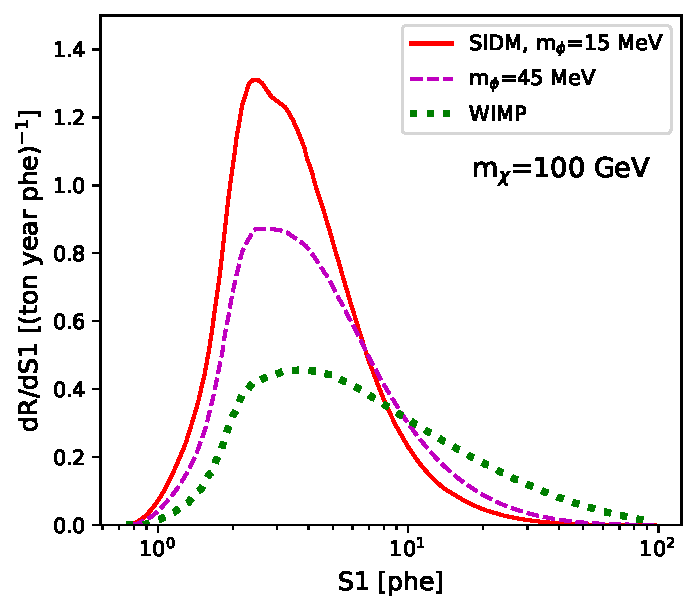
\includegraphics[width=\columnwidth]{fig_sidmspectrum.pdf}
	\caption{Predicted event rates at a xenon-based experiment for a self-interacting dark matter model with a light mediator (solid red), a model with three times the mediator mass (dashed magenta), and the vanilla WIMP model with contact interaction (dotted green). The spectra are normalized to have the same number of total events within the signal range. See~\cite{DelNobile:2015uua} for details.} 
	\label{fig:s1_sidmspectrum}
\end{figure}

Self-interacting dark matter (SIDM)~\cite{Spergel:1999mh,Kaplinghat:2015aga} is a leading candidate that can resolve both long-standing and more recent tensions between small-scale structure observations and prevailing cold dark matter predictions, see~\cite{Tulin:2017ara} for a review. Dark matter self-interactions, analogous to the nuclear interactions, can thermalize the inner Galactic halo in the presence of the stellar component and tie dark matter and baryon distributions in accord with observations~\cite{Kaplinghat:2013xca,Kamada:2016euw,Creasey:2016jaq,Ren:2018jpt}. In many particle physics realizations of SIDM, there exists a light force carrier that mediates dark matter self-interactions~\cite{Feng:2009hw, Buckley:2009in,Loeb:2010gj,Aarssen:2012fx,Tulin:2013teo,Kahlhoefer:2017umn,Chu:2018faw}. When the mediator couples to Standard Model particles, it may generate dark matter signals in direct detection experiments~\cite{Kaplinghat:2013yxa}. For a typical SIDM model, the mediator mass is comparable to or less than the momentum transfer in nuclear recoils. Compared to WIMPs with a contact interaction, the SIDM signal spectrum is then more peaked towards low recoil energies~\cite{DelNobile:2015uua,Kahlhoefer:2017ddj}, see \autoref{fig:s1_sidmspectrum}. Thus the detection of such a spectrum can be an indication of the self-scattering nature of dark matter. Even a null result can put a stringent constraint on the coupling constant between the two sectors. Recently, the PandaX-II collaboration analyzed their data based on an SIDM model with a dark photon mediator and derived an upper bound of $\sim10^{-10}$~\cite{Ren:2018gyx} on the kinematic mixing parameter between the dark and visible photons. Limits from liquid xenon experiments set the strongest constraints also on light SIDM models~\cite{Tsai:2020vpi}. The next-generation liquid xenon experiment discussed in this review will further test SIDM models, and dark matter models with a light mediator in general. 

\subsection{Leptophilic Interactions}

While past efforts in direct dark matter detection have mostly focused on WIMP couplings to nucleons, it is also possible that dark matter would couple preferentially to leptons. Such ``leptophilic'' dark matter candidates have been discussed extensively in the context of the cosmic ray positron excess observed by PAMELA~\cite{Adriani:2013uda} and AMS-02~\cite{Aguilar:2019owu}, as well as the bright $511\1{keV}$ X-ray signal from the Galactic Center~\cite{Knodlseder:2005yq}, and the high-energy cosmic ray electron data from DAMPE~\cite{Ambrosi:2017wek}. Leptophilic dark matter is easily realized in concrete models. This is the case, for instance, if dark matter interactions with the Standard Model particles are mediated by a new gauge boson that couples predominantly to leptons~\cite{Fox:2008kb,Bell:2014tta}. Another example are dark matter interactions mediated by new scalar particles carrying lepton number, such as the sleptons in supersymmetric models~\cite{Chun:2009zx,Bringmann:2012vr,Agrawal:2014ufa,Kopp:2014tsa,Fukushima:2014yia}.

Even if the tree-level interactions of dark matter are leptophilic, couplings to nucleons can be induced at loop level. In that case the WIMP--nucleon scattering is the more promising detection channel, despite loop-suppression, as long as the WIMP is much heavier than the electron~\cite{Kopp:2009et,Schmidt:2012yg,Kopp:2014tsa,Chang:2014tea,Bai:2014osa,Bell:2014tta,Kile:2014jea,Roberts:2016xfw,DEramo:2017zqw}. The reason for this is the more favorable kinematics: the scattering of a heavy WIMP ($\gg \mathrm{MeV}$) on an electron leads to a very small momentum transfer, mostly invisible to a typical direct detection experiment.

However, there are scenarios in which WIMP couplings to nucleons are absent even at the loop level. This can happen for instance if WIMP--lepton interactions are mediated by a new axial vector boson. In this case, the dominant direct detection signal is dark matter scattering on electrons~\cite{Kopp:2009et,Roberts:2015lga,Roberts:2016xfw}, and searches for this process have been carried out by many experiments, including XENON100~\cite{Aprile:2015ade,Aprile:2015ibr,Aprile:2017yea} and LUX~\cite{Akerib:2018zoq}. Scattering on electrons is particularly efficient for sub-GeV dark matter~\cite{Essig:2011nj}, making it the primary detection channel in that mass range. 

Scattering on electrons is also the most efficient channel for dark matter capture in the Sun~\cite{Kopp:2009et,Garani:2017jcj,Liang:2018cjn}. Therefore, if dark matter annihilates into a final state including high-energy neutrinos, searches for these neutrinos from the Sun leads to highly competitive and complementary limits. On the collider side, strong limits on leptophilic dark matter are obtained from LEP data~\cite{Fox:2011fx}. Future lepton collider would lead to further improvements~\cite{Dreiner:2012xm,Freitas:2014jla,Rawat:2017fak}. Progress with these experiments will be complementary to advances from the experiment proposed here.

\subsection{Modulation Searches}

As the Earth revolves around the Sun, a sinusoidal annual modulation should be observable in the dark matter flux hitting direct detection experiments underground~\cite{Drukier:1986tm,Freese:1987wu}. The DAMA/LIBRA collaboration upholds a long-standing claimed observation of an annually modulating event rate~\cite{Bernabei:2018yyw} with a statistical significance in excess of 9$\sigma$. However, most interpretations of this signal in terms of WIMPs have been ruled out by numerous other experiments. A substantial level of particle model fine-tuning is now required to reconcile the DAMA/LIBRA observation with other null results~\cite{Baum:2018ekm}. Moreover, no evidence of a modulation has been found in experiments such as ANAIS~\cite{Amare:2019jul,Amare:2021yyu} and COSINE-100~\cite{Adhikari:2019off,Adhikari:2021szr} which are replicating DAMA/LIBRA with an identical sodium iodide target.

A next-generation liquid xenon experiment will be robustly constructed using long-term infrastructure that is made to last multiple years or even decades. Combined with the extremely low background and large target mass, a next-generation experiment may be the ideal experiment to perform an annual modulation search. An annual modulation analysis thus is an integral part of the primary dark matter data analysis, with a sensitivity enhanced by the long data taking time spanning many annual cycles.

A diurnal modulation is guaranteed for most dark matter candidates due to the varying speed of the Earth relative to the dark matter wind as the Earth rotates, though this will be around two orders of magnitude smaller than the annual modulation. However, if dark matter interacts more strongly inside the Earth, then there may be a much larger diurnal modulation effect as the Earth's ``shadow'' eclipses the dark matter wind from the perspective of an experiment~\cite{Collar:1993ss,Hasenbalg:1997hs,Kavanagh:2016pyr,Emken:2017qmp}. Such shadowing effect also provides additional sensitivity to cosmic-ray boosted dark matter (CRDM) with mass lower than around 1~GeV~\cite{PROSPECT:2021awi}.  Many models within the scope of a future xenon experiment will exhibit such a modulation (\autoref{sec:broaderdarkmatter}).

Experimentally, the challenge for detecting diurnal modulations remains to understand sub-1\% variations in detector parameters on a daily basis rather than from weekly or monthly calibrations. In a massive next-generation detector, spatial variation of quantities such as light collection efficiencies may be inherently greater, but there is no reason to assume that temporal variation will be worse than in contemporary detectors. These experiments can teach us how to better control variation, through existing logging of temperature and pressure data as function of time, and excellent handles for temporal systematic uncertainties~\cite{Mount:2017qzi,Aprile:2017aty}, especially when coupled to frequent calibrations using fast-decaying radioisotopes such as $^{83\textrm{m}}$Kr~\cite{Kastens:2009pa, Manalaysay:2009yq}. 

\subsection{Confronting the Neutrino Fog}\label{sec:nufloor}

As the size and sensitivity of direct detection experiments improves, the detectable signal of dark matter will become so small that it will reach a level similar to the strength of the coherent elastic neutrino-nucleus scattering signal of astrophysical neutrinos~\cite{Monroe:2007xp,Strigari:2009bq,Billard:2013qya}. While there is a substantial science case for the detection of astrophysical neutrinos in their own right (\autoref{sec:neutrinos}), for dark matter searches they are a critical background.

When searching for a signal that is mimicked by a background, discovery is only possible when an excess in events is larger than the expected statistical fluctuations and systematic uncertainties of that background. For the neutrino background, the systematic uncertainties on the flux normalizations dominate, which range from 1\%--50\%. Many of the particle models discussed here will eventually be limited in some way by the neutrino background, in both the electronic~\cite{Wyenberg:2018eyv,Essig:2018tss} and nuclear recoil channels~\cite{Billard:2013qya,Baudis:2013qla,Dent:2016iht,Dent:2016wor,Dent:2019krz}. These limits are generally referred to as ``neutrino floor’’, or ``neutrino fog''. Just like any generic limit on dark matter, the shape of a neutrino fog is dependent on nuclear~\cite{Papoulias:2018uzy}, astrophysical~\cite{OHare:2016pjy} and particle model~\cite{Dent:2016iht,Dent:2016wor,Gelmini:2018ogy} inputs for the dark matter signal. Given non-standard neutrino-nucleus interactions, these could be further modified~\cite{AristizabalSierra:2017joc,Gonzalez-Garcia:2018dep} and even raised by several orders of magnitude~\cite{Boehm:2018sux}.

Unlike many other backgrounds, neutrinos cannot be shielded, so they must be dealt with statistically, or by searching for some discriminating features. Techniques that have been discussed in the past include exploiting the differing annual modulation signatures~\cite{Davis:2014ama}, or the complementarity between different target nuclei~\cite{Ruppin:2014bra}. However, only direction-dependence provides enough of a discriminant to fully subtract the background~\cite{Grothaus:2014hja,O'Hare:2015mda,Mayet:2016zxu,Franarin:2016ppr,OHare:2017rag}, but measuring this in any large-scale experiment is extremely challenging. 

\begin{figure}[!htbp]
\begin{center}
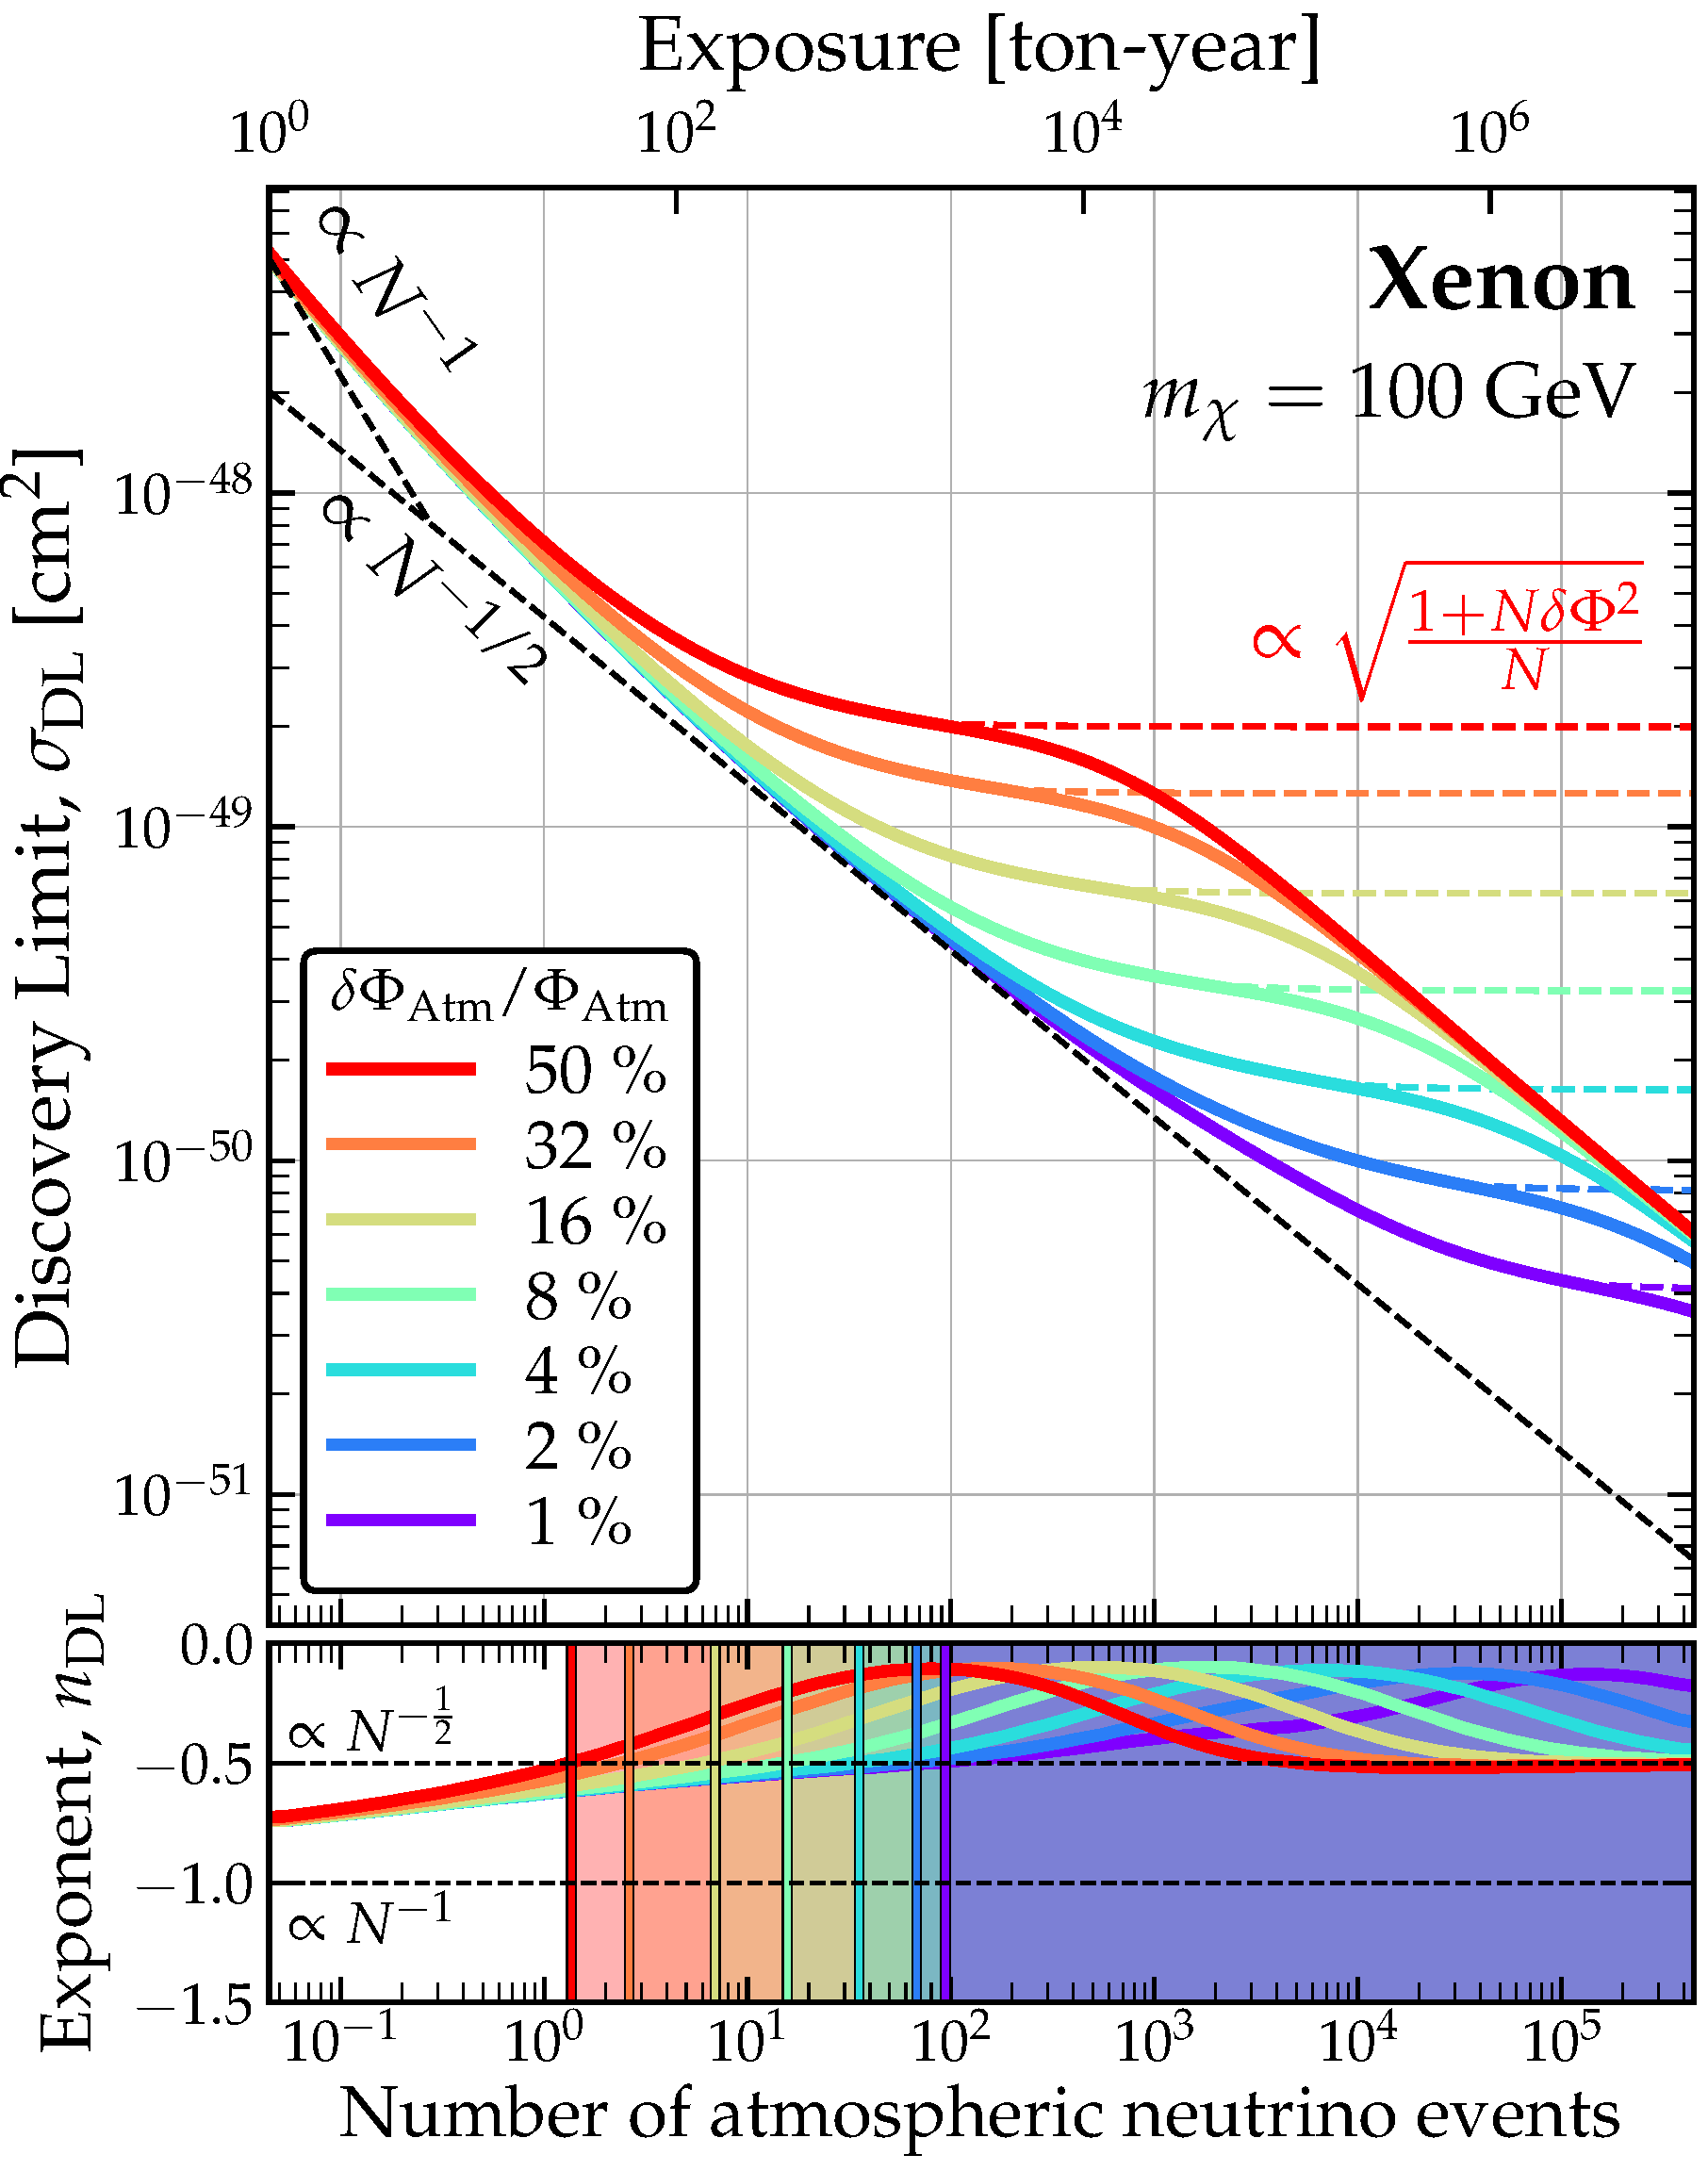
\includegraphics[width=0.98\columnwidth]{fig_nufloor_100GeV.pdf}
\caption{Spin-independent discovery limits at $m_\chi = 100$~GeV as a function of the expected number of atmospheric CEvNS events $N$, and the fractional uncertainty on the atmospheric neutrino flux, $\delta \Phi_{\rm Atm}/\Phi_{\rm Atm}$ from~\cite{OHare:2016pjy}. Three scaling regimes as a function of $N$ are shown with dashed lines: 1) ``background-free'' $\sigma \sim N^{-1}$, 2) Poissonian $\sigma \sim N^{-1/2}$, and 3) Saturation $\sigma \sim \sqrt{(1+\delta\Phi^2 N)/N}$. The bottom panels in each case show the logarithmic scaling exponent defined as: $n_{\rm DL} \equiv \textrm{d} \ln\sigma_{\rm DL}/\textrm{d} \ln N$. This figure shows the importance of the neutrino flux systematic uncertainty in extending the dark matter physics reach below the neutrino fog.}
\label{fig:fig_nufloor_100GeV}
\end{center} 
\end{figure}

Fortunately for the next-generation xenon experiment, extending the dark matter physics reach below the neutrino fog will be facilitated by complementary measurements made by neutrino experiments. Taking the example of standard WIMP-nucleon cross sections, the most important backgrounds will be $^8$B solar neutrinos for WIMP masses below $\sim$10\,GeV/$c^2$, and atmospheric neutrinos above that. The $^8$B flux is measured at the 2\% level from Solar neutrino data~\cite{Bergstrom:2016cbh}. The atmospheric flux on the other hand, is difficult to measure and theoretically predict at the relevant sub-100~MeV energies, so it still has a $\sim$20\% uncertainty (\autoref{sec:atmnu} and~\cite{Newstead:2020fie}). Any reduction in these uncertainties will in effect ``lower’’ the neutrino fog. Indeed, gradual improvements in neutrino flux measurements are expected independently of the experiment under discussion here. For example, experiments like SNO+~\cite{Caden:2017htb}, JUNO~\cite{JinpingNeutrinoExperimentgroup:2016nol} and DUNE~\cite{Abi:2018dnh,Kelly:2019itm} will be either operating or under construction over a similar timescale to the next-generation xenon experiment.

In \autoref{fig:fig_nufloor_100GeV} we show how the minimum discoverable spin-independent cross section for a $100\1{GeV}$ WIMP evolves with increasing exposure in a xenon experiment. The brief plateau in the discovery limit is the impact of the atmospheric neutrino background. However, in the limit of high statistics, the number of observed background events will eventually be large enough to account for the finite uncertainty. At this point, the discovery limit breaks past the neutrino fog and smaller cross sections can be accessed. Comparing the different lines, we see clearly the importance of the systematic uncertainty. A future improvement down to $\sim$4\% would be enough to extend the reach of a 1000~tonne-year xenon experiment almost an order of magnitude into the neutrino fog at high masses~\cite{OHare:2020lva}. This is where much of the remaining supersymmetric WIMP candidates~\cite{Roszkowski:2014iqa,Athron:2017qdc,Hisano:2011cs,Kobakhidze:2018vuy}, as well as many alternative WIMP models~\cite{Arcadi:2017wqi,Baker:2019ndr,Arina:2019tib} lie.

